\documentclass[12pt,twoside]{report}
\setcounter{secnumdepth}{3}

\usepackage[utf8]{inputenc}
\usepackage{hyperref}
\usepackage{graphicx}
\usepackage[a4paper,width=150mm,top=25mm,bottom=25mm,bindingoffset=6mm]{geometry}
\usepackage[pagestyles]{titlesec}
\usepackage{lipsum}
\usepackage{tikz}
\usepackage{float}
\usepackage{booktabs}
\usepackage{csquotes}
\usepackage{amsmath}
\usepackage{amsthm}
\usepackage{enumitem}
\usepackage{datetime}
\usepackage{subcaption}
\usepackage[titletoc]{appendix}
\usepackage{titlesec}
\usepackage{enumitem}
\usepackage{listings}
\usepackage{soul}
\usepackage{multirow}
\usepackage{array}
\usepackage{url}

\counterwithout{footnote}{chapter}

\makeatletter
\newcommand\footnoteref[1]{\protected@xdef\@thefnmark{\ref{#1}}\@footnotemark}
\makeatother

\usetikzlibrary{shapes,arrows,trees,positioning}
\tikzstyle{block}=[draw, fill=blue!20, minimum size=2em]
\tikzstyle{inter}=[draw, fill=gray!20, minimum size=2em]

\hypersetup{
    colorlinks=true,
    linkcolor=blue,
    filecolor=magenta,
    urlcolor=blue,
    citecolor=blue
}

\lstset{
	columns=fullflexible,
 	breaklines=true,
	postbreak=\mbox{\textcolor{red}{$\hookrightarrow$}\space},
	numbers=left,
	numberstyle=\tiny\color{blue},
	language=Prolog,
	showstringspaces=false
}

% https://tex.stackexchange.com/questions/81942/div-equivalent-to-mod
\makeatletter
\newcommand*{\bdiv}{%
  \nonscript\mskip-\medmuskip\mkern5mu%
  \mathbin{\operator@font div}\penalty900\mkern5mu%
  \nonscript\mskip-\medmuskip
}
\makeatother

% https://tex.stackexchange.com/questions/7032/good-way-to-make-textcircled-numbers
%\newcommand*\circled[1]{\tikz[baseline=(char.base)]{
            %\node[shape=circle,draw,inner sep=2pt] (char) {#1};}}
\newcommand*\circled[1]{\raisebox{.5pt}{\textcircled{\raisebox{-.9pt} {#1}}}}

\newpagestyle{Headings}{
 \sethead
   {Chapter \thechapter: \chaptertitle}
   {}
   {Section \toptitlemarks\thesection: \toptitlemarks\sectiontitle}
   \headrule
 \setfoot{}{\thepage}{}
}
\newpagestyle{PageNum}{
 \setfoot{}{\thepage}{}
}

\theoremstyle{definition}
\newtheorem{definition}{Definition}
\newtheorem{objective}{Objective}
\newtheorem{contribution}{Contribution}

\newcommand{\tabitem}{~~\llap{\textbullet}~~}
\newcommand{\floor}[1]{\lfloor #1 \rfloor}

% https://tex.stackexchange.com/questions/54069/table-with-text-wrapping/414580
\newcolumntype{L}[1]{>{\raggedright\let\newline\\\arraybackslash\hspace{0pt}}p{#1}}

\graphicspath{ {media/} }

\newcommand{\reporttitle}{Using Answer Set Grammars For Text Summarization}
\newcommand{\reportauthor}{Julien Amblard}
\newcommand{\supervisor}{Alessandra Russo}
\newcommand{\cosupervisor}{David Tuckey}
\newcommand{\secondmarker}{Krysia Broda}
\newcommand{\reporttype}{Individual Project}
\newcommand{\degreetype}{Computing MEng}

\begin{document}

\pagenumbering{roman}

\pagestyle{empty}
% Last modification: 2015-08-17 (Marc Deisenroth)
\begin{title}

\newcommand{\HRule}{\rule{\linewidth}{0.5mm}} % Defines a new command for the horizontal lines, change thickness here

%----------------------------------------------------------------------------------------
%	LOGO SECTION
%----------------------------------------------------------------------------------------

\includegraphics[width = 4cm]{imperial_logo.eps}\\[0.5cm] 

\center % Center everything on the page
 
%----------------------------------------------------------------------------------------
%	HEADING SECTIONS
%----------------------------------------------------------------------------------------

\textsc{\LARGE \reporttype}\\[1.5cm] 
\textsc{\Large Department of Computing}\\[0.5cm] 
\textsc{\large Imperial College of Science, Technology and Medicine}\\[0.5cm] 

%----------------------------------------------------------------------------------------
%	TITLE SECTION
%----------------------------------------------------------------------------------------

\HRule \\[0.4cm]
{ \huge \bfseries \reporttitle}\\ % Title of your document
\HRule \\[1.5cm]
 
%----------------------------------------------------------------------------------------
%	AUTHOR SECTION
%----------------------------------------------------------------------------------------

\begin{figure}[H]
	\begin{minipage}[t]{0.49 \linewidth}
		\large\emph{Author:}\\
		\reportauthor
	\end{minipage}
	\begin{minipage}[t]{0.49 \linewidth}
	\begin{flushright}
 		\large\emph{Supervisor:} \\
		\supervisor
	\end{flushright}
	\end{minipage}
\end{figure}
	
\begin{figure}[H]
	\begin{minipage}[t]{\linewidth}
	\begin{flushright}
 		\large\emph{Co-Supervisor:} \\
		\cosupervisor
	\end{flushright}
	\end{minipage}
\end{figure}
	
\begin{figure}[H]
	\begin{minipage}[t]{\linewidth}
	\begin{flushright}
 		\large\emph{Second Marker:} \\
		\secondmarker
	\end{flushright}
	\end{minipage}
\end{figure}

\mbox{}

%----------------------------------------------------------------------------------------


%----------------------------------------------------------------------------------------
%	DATE SECTION
%----------------------------------------------------------------------------------------

{\large \today} % Date, change the \today to a set date if you want to be precise


\vfill % Fill the rest of the page with whitespace
Submitted in partial fulfillment of the requirements for the \degreetype~of Imperial College London

\end{title}


\abstract{
\thispagestyle{plain}
To this day, text summarization remains a largely open-ended problem in Natural Language Processing, and is most often resolved using some form of Machine Learning.

In this project, we aim to resolve the problem for short texts about a paragraph in length, via a novel approach that makes use of Answer Set Grammars. By combining ideas from the fields of logic-based learning, knowledge representation and linguistics, we have created a system that is capable of producing partially \textit{abstractive}, \textit{generic} and \textit{informative} summaries, as well as scoring them by order of pertinence and information density.

The approach chosen for this project relies on a central context-free grammar as its internal representation for a simplified version of the English language. Using Answer Set Programming, the system is able to perform logic-based learning to understand the input text after having pre-processed it, the result of which then goes through a number of summarization logic rules, producing a set of possible summaries.

Throughout the development phase, we ran our system on a suite of targeted examples. When the implementation was complete, we successfully trained a neural network to learn the summarization rules used by our framework, thereby validating our approach. We then performed two experiments to evaluate our system, and to establish some of the key differences compared to a neural network.

From this we conclude that although our approach is less general than a neural network, it is able to produce more consistent results and can detect grammatically-incorrect text. Moreover, it does not rely on noisy annotated data, and can be expanded upon without the need to be retrained.
}
\setcounter{page}{2}
\newpage

\newenvironment{acknowledgements}
    {\thispagestyle{plain}\null\vfill\begin{center}
    \bfseries Acknowledgements\end{center}}
    {\vfill\null}
        \begin{acknowledgements}
        Firstly, I would to thank my supervisor Prof. Alessandra Russo, as well as my co-supervisor David Tuckey, for the time they have put into this project. Week after week, we have had very interesting discussions in which they have provided their respective expertise in logic programming and NLP, helping to move the project forward. I would also like to thank Mark Law for creating ASG, as well as helping we with some of the syntax and numerous optimizations. In addition, I would like to thank my Personal Tutor, Antonio Filieri, for providing advice and guidance throughout my four years at Imperial. Finally, I am grateful for my family who supported me during my studies.
        \end{acknowledgements}
\newpage

\floatstyle{boxed}
\restylefloat{figure}

\pagestyle{PageNum}
\tableofcontents
\thispagestyle{PageNum}

\newpage

\titleformat{\chapter}
{\normalfont\huge}{\chaptertitlename{} \thechapter}{20pt}{\bfseries\huge}
\titlespacing*{\chapter}{0pt}{0pt}{40pt}

\pagestyle{Headings}
\pagenumbering{arabic}

\chapter{Introduction}
\label{chapter:introduction}

In general, the task of summarization in Natural Language Processing (NLP) is to produce a shortened text which covers the main points expressed in a longer text given as input. To this end, a system performing such a task must analyse and process the input in order to extract from it the most important information.

\section{Motivations}

In recent years, state-of-the-art systems that accomplish text summarization have relied largely on Machine Learning. These include Bayesian classifiers, hidden Markov models, neural networks and fuzzy logic, among others \cite{kiyani_survey_2017}. Given a training corpus, along with some careful pre-processing as well as fine-tuning of hyper-parameters and feature extraction functions, such systems are able to produce effective summaries \cite{kiyani_survey_2017}.

Among these approaches, one of the most prominent types of neural networks is the \textit{encoder-decoder}. These are commonly used for sequence-to-sequence translation due to their promising performance in NLP tasks \cite{yao_dual_2018}. \textit{encoder-decoders} use a fixed-dimension internal representation which can be trained to act as an intermediate between variable-length inputs and outputs, making this approach highly suitable for text summarization. However to learn what is a summary, these systems require tremendous amounts of data and take a long time to train.

In our case, using logic means that we can hard-code the definition of a summary directly into the program, avoiding the problem of randomness and uncertainty that often comes with neural networks. By carefully constructing the structure of our system, we can get results with just a short list of rules, and know that it will always produce a complete and valid output with respect to the background knowledge we encode into it.

\section{Objectives}

The main goal of this project is to explore the task of text summarization via logic-based learning with Answer Set Grammars (ASG). Below you will find the principal objectives which were established as being vital to achieving this goal.

\begin{objective}[Translate English Into ASG]
Our system should be capable of taking a text written in English and converting it into some logic-based form that can be interpreted by ASG. Moreover, this representation should capture as much of the semantics from the original text as possible, and not be limited to a particular domain.
\end{objective}

\begin{objective}[Generate Summaries Automatically]
Given a brief paragraph of text, for example a short story aimed at young children, we should be able to provide a grammatically correct summary in multiple sentences. This should be fully-automated and not require any human intervention during the process.
\end{objective}

\begin{objective}[Evaluate The Approach]
Once we have implemented the basic approach, we should run our system on a suite of examples to verify that it can produce summaries that closely resemble the corresponding human-generated ones. On a larger scale, it is important to also run it against a popular summarization approach to ensure the sanity of our logic-based mechanism.
\end{objective}

\section{Approach Overview}
\label{sec:approach_overview}

The approach described in this paper, known as \textsc{SumASG*}, can be diagrammatically represented as a three step pipeline, as seen in Figure \ref{fig:main_pipeline}. While the core part of the the project is written in ASG, Python scripts are used to respectively pre-process and post-process the input and output.

{
\floatstyle{plain}
\restylefloat{figure}
\begin{figure}[H]
\centering

\begin{tikzpicture}[node distance=0.3cm, auto]
\node (story) [] {Story};
\node (preprocessor) [block, right =of story] {Preprocessor};
\node (asg) [block, right =of preprocessor] {SumASG};
\node (score) [block, right =of asg] {Post-Processing/Scoring};
\node (summaries) [right =of score] {Scored Summaries};
\draw [->] (story) -- (preprocessor);
\draw [->] (preprocessor) -- (asg);
\draw [->] (asg) -- (score);
\draw [->] (score) -- (summaries);
\end{tikzpicture}
\caption{Main pipeline for \textsc{SumASG*}}
\label{fig:main_pipeline}
\end{figure}
}

\noindent
As the first step in the pipeline, the \textsc{Preprocessor} plays an essential role. Given an input story, its goal is to simplify the story's sentences into a simpler and more consistent structure, one that will then be easier to parse by ASG. Additionally, the \textsc{Preprocessor} removes irrelevant sentences from the story and reduces it lexical diversity, which helps increase the chances of generating a high-quality summary.

Once the story has been pre-processed, it then goes through a procedure we call \textsc{SumASG}. This revolves around a purpose-built internal representation of English sentences, represented as a tree. The first of two steps, \textsc{SumASG\textsubscript{1}}, involves translating sentences from the input story into our internal representation using ASG's learning abilities. From this, \textsc{SumASG\textsubscript{2}} then exploits a number of logic-based rules to generate sentences which may be used to form a summary.

The third and final step in the pipeline serves to turn the output of \textsc{SumASG} into usable summaries. To begin, we post-process the summary sentences given to us as output, and combine them in different ways so as to form potential summaries. Afterwards we assign to each one a score, and only those with the highest scores are returned.

\subsection*{Example}

Throughout this paper, we use the example of the story of Peter Little to illustrate the different steps of our pipeline, as shown below in Figure \ref{fig:peter_little}.

Additional examples of stories can be found in Appendix \ref{appendix:stories}, along with the summaries generated by \textsc{SumASG*}.

\begin{figure}[H]
\begin{subfigure}{\textwidth}
\begin{displayquote}
There was a curious little boy named Peter Little. He was interested in stars and planets. So he was serious in school and always did his homework. When he was older, he studied mathematics and quantum physics. He studied hard for his exams and became an astrophysicist. Now he is famous.
\end{displayquote}
\caption{Original story}
\vspace{\baselineskip}
\end{subfigure}
\begin{subfigure}{\textwidth}
\begin{displayquote}
\textbf{A.} Peter Little was interested in space so he studied hard and became a famous astrophysicist.\\
\textbf{B.} Peter Little was curious about astronomy. He was always serious in school, and now he is famous.
\end{displayquote}
\caption{\textit{Reference summaries}}
\end{subfigure}
\caption{Example of the task of summarization for the story of Peter Little}
\label{fig:peter_little}
\end{figure}

\section{Contributions}

The main contribution of this project to the field of NLP is the creation of an end-to-end, fully-automated logic-based system capable of text summarization, without the need of any training whatsoever, as would be the case with a typical Machine Learning-based approach these days. Going more into depth, we discuss some more specific contributions in what follows.

\begin{contribution}[Identification Of Existing Techniques Used For Summarization]
After researching existing state-of-the-art text summarization systems, identified techniques which were beneficial to use for this project (e.g., \textit{text relationship maps}).
\end{contribution}

\begin{contribution}[Complexity Reduction In Some English Sentences]
Implemented an algorithm that dramatically reduces the complexity in the structure of certain English sentences, without losing too much information (e.g., co-referencing).
\end{contribution}

\begin{contribution}[Removal Of Irrelevant Sentences And Homogenization]
Implemented an algorithm which uses \textit{similarity} to remove irrelevant sentences from a short story, and replaces synonyms with a single representative in each set of synonyms.
\end{contribution}

\begin{contribution}[Representation Of English In ASG]
Created a context-free grammar that models the structure of basic English sentences, and can be used both for semantic learning, as well as generating grammatically-correct text.
\end{contribution}

\begin{contribution}[Translation Of English Into ASG]
Wrote an ASG learning task capable of taking English text and turning it into set of chronologically-ordered \textit{actions} which convey in ASP what occurs in the text.
\end{contribution}

\begin{contribution}[Automatic Generation Of Summaries]
Developed a set of rules which, given \textit{actions} from a story, allow ASG to generate both \textit{extractive} and \textit{abstractive} summary sentences.
\end{contribution}

\begin{contribution}[Scoring Mechanism]
Implemented a scoring mechanism prioritizing information density, while taking into account words which may appear frequently in English and can be considered the \textit{topic} of the original text.
\end{contribution}

\section{Paper Structure}

In this paper, we begin by discussing some essential background knowledge in Chapter \ref{chapter:background}. After giving an overview of text summarization, we introduce the notion of \textit{syntactic parsing}. Then, we go over some concepts that will be necessary in order to understand the ASG part of the pipeline. Finally, we briefly mention some Machine Learning structures which we make use of for evaluating our implementation.

In Chapters \ref{chapter:preprocessor}, \ref{chapter:asg} and \ref{chapter:postprocessing}, we dive into the various steps involved in the pipeline of \textsc{SumASG*}, as outlined in Section \ref{sec:approach_overview}. In addition, we discuss possible technical improvements for each step of the pipeline in Chapter \ref{chapter:improvements}.

After this, we show in Chapter \ref{chapter:evaluation} that our system is capable of producing a more consistent output and is more easily expandable than an \textit{encoder-decoder} trained for text summarization.

In Chapter \ref{chapter:related_work} we explore some of the existing state-of-the-art implementations and differentiate between statistical, frame and symbolic approaches. Where relevant, we discuss which ideas from these approaches we have borrowed for \textsc{SumASG*}, as well as how our approach differs from these implementations.

Finally, we conclude the paper in Chapter \ref{chapter:conclusion} by listing the main achievements of this project, as well as giving a high-level overview of future work which may be done to build on \textsc{SumASG*}.

\chapter{Background}
\label{chapter:background}

\section{Summarization}

\subsection{Definition} \label{sec:definition}

As described by the author in \cite{lloret_text_2008}, a summary is a way of providing a large part of the information contained in one or more original passages, using at most half of the text. Summaries can be grouped into one of the two following categories:

\begin{itemize}[nolistsep]
\item An \textit{extract} is made up of sentences which are copied word-for-word.
\item An \textit{abstract} is a rewriting of the original text's content in a more concise form.
\end{itemize}

\mbox{}

A different way to group summaries is the following:

\begin{itemize}[nolistsep]
\item \textit{Generic} summaries do not try and focus on anything in particular, they simply aim to recount the most important features.
\item \textit{Focused} (or \textit{query-driven}) summaries, on the other hand, require a user-input, which specifies the focus of the summary. For this project, we may want to introduce a bias to our learning program, so that we end up with a summary which meets a certain number of criteria. For instance, we might want it to ensure it captures at least one action verb from the original passage.
\end{itemize}

\mbox{}

Yet another way \cite{radev_introduction_2002} is shown below, with examples given in Figure \ref{fig:indicative_informative_summaries}:

\begin{itemize}[nolistsep]
\item \textit{Indicative} summaries give the overall impression of a text, but without conveying any details.
\item \textit{Informative} summaries, on the other hand, take the content from an original document and give a shortened version of it.
\end{itemize}

\begin{figure}[H]\
\begin{subfigure}{\textwidth}
\begin{displayquote}
It’s going to be windy across the western half of the UK, with gusts reaching 60 to 70mph along Irish Sea coastlines, the west of Scotland and perhaps some English Channel coasts. Those in affected areas are advised to take extra care when driving on bridges or high open roads. Flood warnings were issued on Sunday for two areas – Keswick campsite in Cumbria and a stretch along the River Nene east of Peterborough.
\end{displayquote}
\caption{\textit{Indicative} summary}
\vspace{\baselineskip}
\end{subfigure}
\begin{subfigure}{\textwidth}
\begin{displayquote}
Yellow warnings of strong winds were put in place for parts of the UK. These very strong winds are likely to cause travel disruption, so those in affected areas are advised to take extra care when driving on exposed routes. In addition, heavy rain is expected in parts of the country, which could cause local flooding.
\caption{\textit{Informative} summary}
\end{displayquote}
\end{subfigure}
\caption{Example of \textit{indicative} and \textit{informative} summaries for a \href{https://www.theguardian.com/uk-news/2020/jan/12/storm-brendan-gales-forecast-uk}{news article}}
\label{fig:indicative_informative_summaries}
\end{figure}

\subsection{Summarization Levels}

Depending on how much text analysis is done, we identify three different levels of summarization \cite{lloret_text_2008}. Many current systems employ what is called a \textit{hybrid approach}, combining techniques from different levels.

\subsubsection{Surface Level}

On a \textit{surface level}, little analysis is performed, and we rely on keywords in the text which are later combined to generate a summary. Techniques which are common include:

\begin{itemize}
\item \textit{Thematic features} are identified by looking at the words that appear the most often. Usually, the important sentences in a passage have a higher probability of containing these \textit{thematic features}.
\item Often, the \textit{location} of a sentence can help identify its importance; the first and last sentences are generally a good indicator for the respective introduction and conclusion of a document. Moreover, we may want to make use of the title and heading (if any) to find out which topics are most relevant.
\item \textit{Cue words} are expressions like ``in this article" and ``to sum up"; these can give us a clue as to where the relevant information is.
\end{itemize}

\subsubsection{Entity Level}

A more analytic approach can be done at an \textit{entity level}, where we build a model of a document's individual entities and see how they relate. Common techniques include:

\begin{itemize}
\item \textit{Similarity} between different words (or phrases), whether it be synonyms or terms relating to the same topic.
\item \textit{Logical relations} involve the use of a connector such as ``before" or ``therefore", and tell us how the information given by such connected phrases relates.
\end{itemize}

\subsubsection{Discourse Level}

Finally at a \textit{discourse level} we go beyond the contents of a text, exploiting its structure instead. Some of the things we can analyze are:

\begin{itemize}
\item The \textit{format} can be taken into account to help us extract key information. For example, in a rich-text document we may want to pay close attention to terms that are underlined or italicized.
\item The \textit{rhetorical structure} can tell us whether the document is argumentative or narrative in nature. In the latter case a more concise description of the text's contents would suffice, while the former would involve recounting the key points and conclusions made by the author.
\end{itemize}

\section{Syntactic Parsing}

Given a text, \textit{syntactic parsing} \cite{noauthor_syntactic_nodate} describes the process of tokenization, whereby the grammatical link between parts of speech is established. Two of the most prominent syntactic parsers are \textbf{\href{https://corenlp.run}{CoreNLP}} (developed by Stanford) and \textbf{\href{https://spacy.io}{spaCy}}.

This tokenization can then be visualized in the form of a \textit{parse tree}, which makes it possible to identify different parts of speech, such as nouns, verbs and adjectives. Additionally, each of these \textit{tokens} is assigned a \textit{lemma}, which is essentially the ``neutral" form for a word, be it the singular of a noun or the base form of a verb.

Example \textit{parse trees} are shown in Table \ref{table:basic_sentence} for both of the mentioned parsers. Appendix \ref{appendix:pos} shows how to interpret position of speech (POS) tags.

\begin{table}[H]
\centering
\begin{tabular}{@{}ll@{}}
\toprule
\textbf{CoreNLP} & 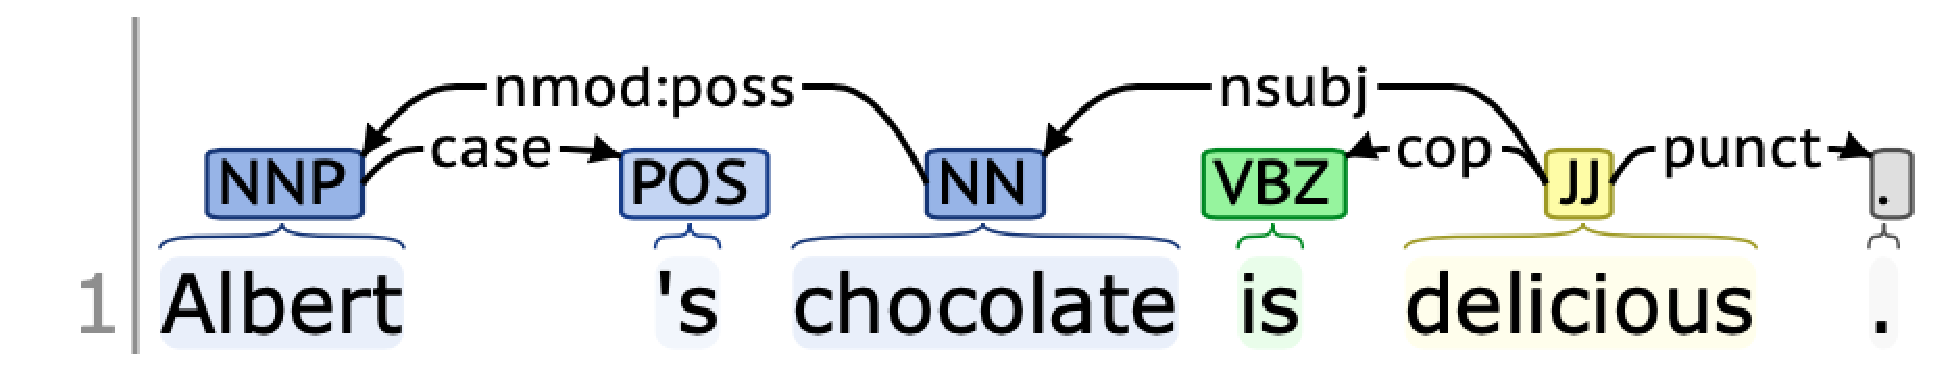
\includegraphics[width=0.75\textwidth]{basic_sentence_core_nlp.eps} \\ \midrule
\textbf{spaCy} & 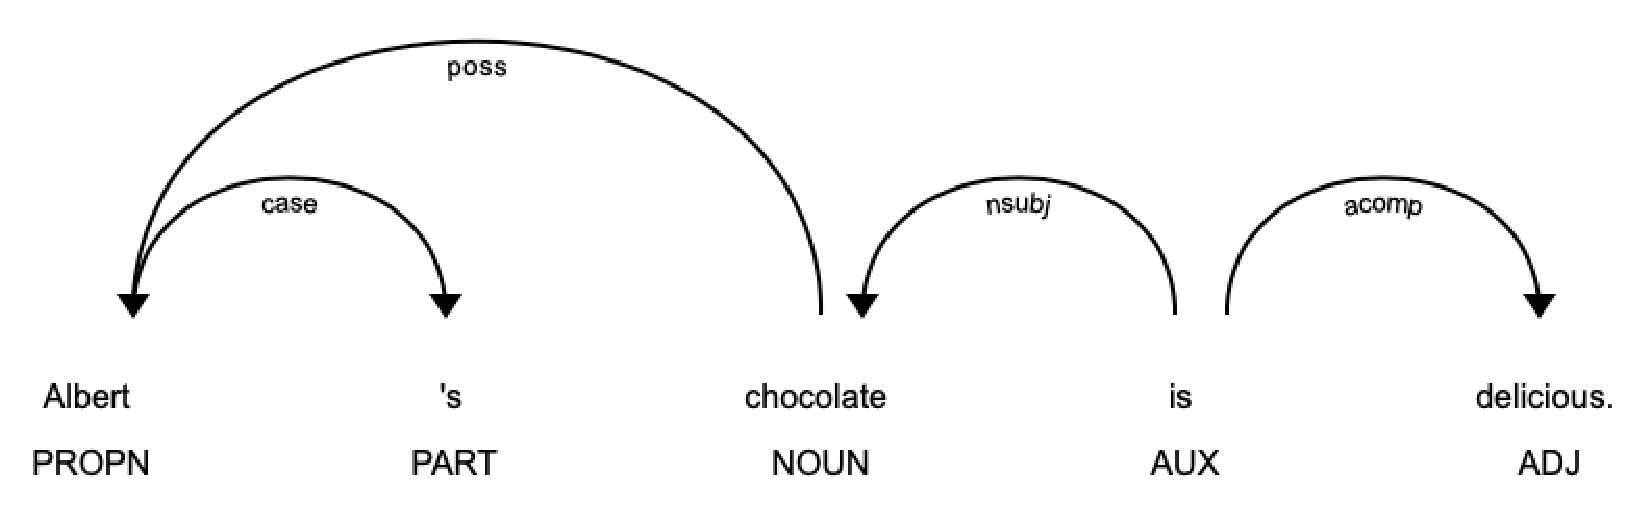
\includegraphics[width=0.85\textwidth]{basic_sentence_spacy.eps}  \\ \bottomrule
\end{tabular}
\caption{Semantic parsing example for a basic sentence}
\label{table:basic_sentence}
\end{table}

However, the English language can often be ambiguous and highly context-dependent, meaning that multiple \textit{parse trees} for the same sentence could emerge. Consider the following two sentences \cite{noauthor_studying_nodate}:
\begin{displayquote}
He fed her cat food. \\
I saw a man on a hill with a telescope.
\end{displayquote}
As shown in Table \ref{table:ambiguous_sentence}, both parsers interpret the meaning of the first example sentence as a person who feeds their ``cat food", which, in addition of not being very logical, is also grammatically incorrect as the genders do not match. Unfortunately, computers are generally not very good at context-based inference, something to take into account for this research project.

Therefore, accuracy is very important for \textit{syntactic parsing} \cite{gomez-rodriguez_how_2019}.

\begin{table}[H]
\centering
\begin{tabular}{@{}ll@{}}
\toprule
\textbf{CoreNLP} & 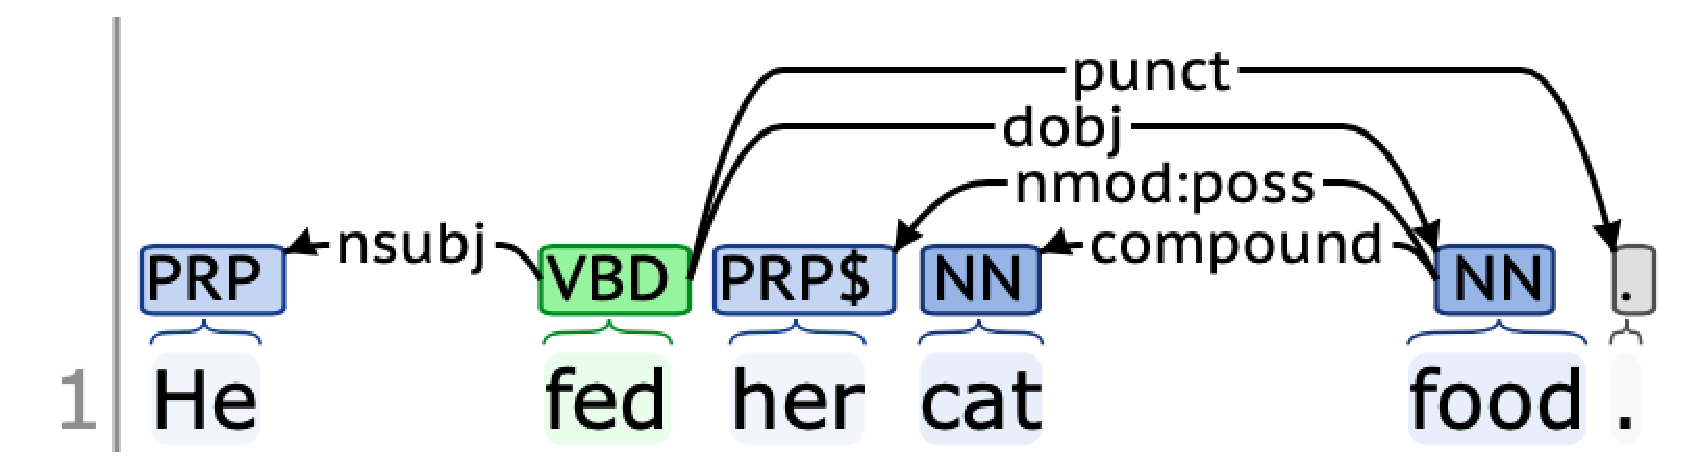
\includegraphics[width=0.75\textwidth]{ambiguous_sentence_core_nlp.eps} \\ \midrule
\textbf{spaCy} & 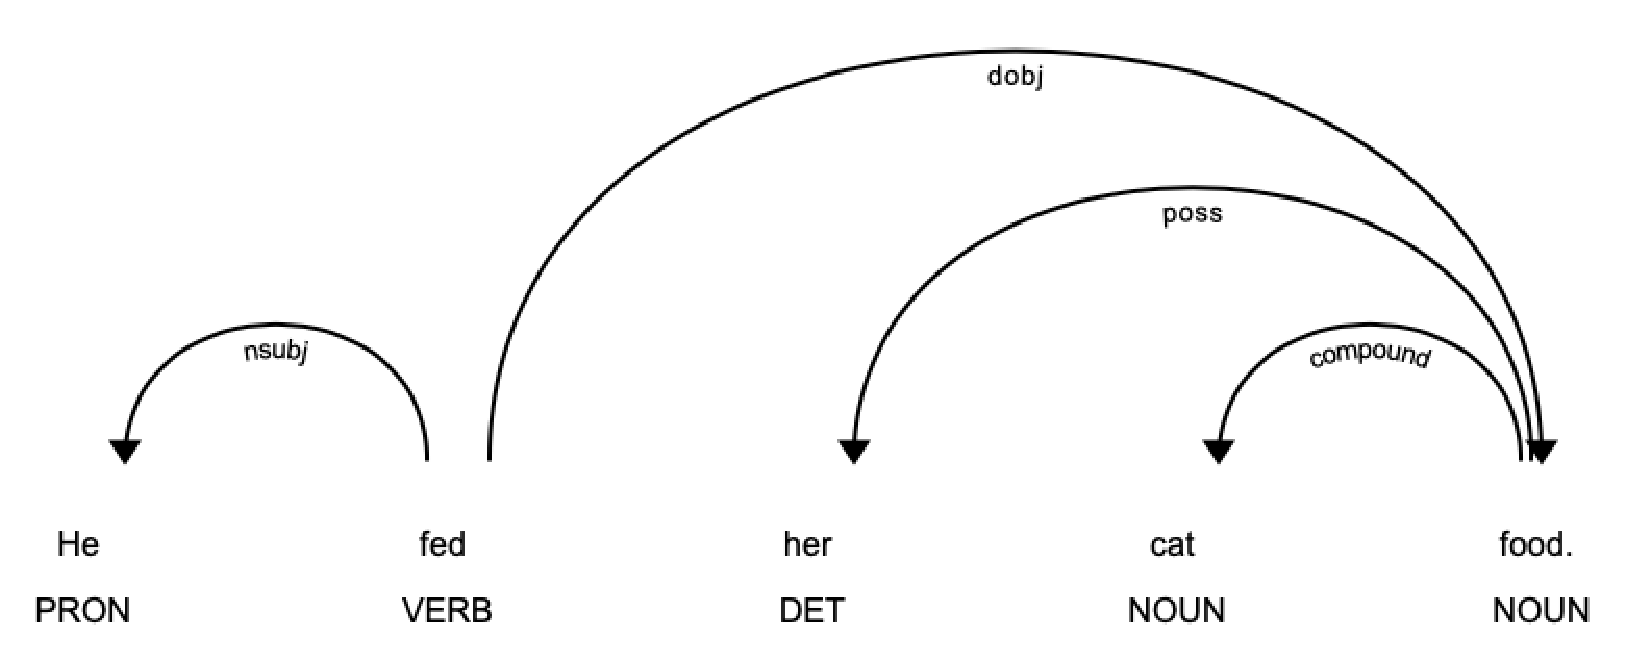
\includegraphics[width=0.85\textwidth]{ambiguous_sentence_spacy.eps}  \\ \bottomrule
\end{tabular}
\caption{Semantic parsing example for an ambiguous sentence}
\label{table:ambiguous_sentence}
\end{table}

\section{Logic Programming}

\begin{definition}[Term \cite{kowalski_predicate_1974}]
A \textit{term} is either a \textit{variable} $x,y,z,...$ or an expression $f(t_1,t_2,...,t_k)$, where $f$ is a k-ary \textit{function symbol} and the $t_i$ are \textit{terms}. A \textit{constant} is a 0-ary \textit{function symbol}.
\end{definition}

\begin{definition}[Atom \cite{kowalski_predicate_1974}]
An \textit{atomic formula} (or \textit{atom}) has the form $P(t_1,t_2,...,t_k)$, where $P$ is a k-ary predicate (boolean function) symbol and the $t_i$ are terms.
\end{definition}

\subsection{Answer Set Programming}

Once we have parsed a text, the next step is to convert this into an answer set program (ASP).

ASP is a declarative first-order (predicate) logic language whose aim is to solve complex search problems \cite{lifschitz_what_nodate}. It is built upon the idea of stable model (answer set) semantics, returns answer sets when asked for the solution to a problem.

In ASP, a \textit{literal} is an \textit{atom} \textit{a} or its negation \textit{not a} (we call this negation as a failure). ASP programs are composed of a set of \textit{normal rules}, whose head is a single \textit{atom} and body is a conjunction of \textit{literals} \cite{law_representing_2019}.
\begin{equation}
h \leftarrow b_1, b_2, ..., b_k, \text{not}\ b_{k+1}, ..., \text{not}\ b_m.
\end{equation}

If the body is empty ($k = m = 0$) then a rule is called a \textit{fact}. We can also have \textit{constraints}, which are like \textit{normal rules} except that the head is empty. These prevent any answer sets from both including $b_1, b_2, ..., b_k$ and excluding $b_{k+1}, ..., b_m$.

\begin{definition}[Safety \cite{law_representing_2019}]
A variable in a rule is said to be \textit{safe} if it occurs in at least one positive \textit{literal} (i.e., the $b_i$s in the above rule) in the body of the rule.
\end{definition}

\begin{definition}[Herbrand Base \cite{law_representing_2019}]
The \textit{Herbrand base} of a program P, denoted $HB_P$, is the set of variable-free (\textit{ground}) \textit{atoms} that can be formed from predicates and \textit{constants} in P. The subsets of $HB_P$ are called the (Herbrand) \textit{interpretations} of P.
\end{definition}

\begin{definition}[Satisfiability \cite{law_representing_2019}] 
\label{def:satisfiability}
Given a set $A$, a \textit{ground normal rule} of P is \textit{satisfied} if the head is in $A$ when all positive \textit{atoms} and none of the negated \textit{atoms} of the body are in $A$, that is when the body is \textit{satisfied}. A \textit{ground constraint} is \textit{satisfied} when the body is not \textit{satisfied}.
\end{definition}

\begin{definition}[Reduct \cite{law_representing_2019}]
Given a program P and a \textit{Herbrand interpretation} $I \subseteq HB_P$, the \textit{reduct} $P^I$ is constructed from the grounding of P in three steps:
\begin{enumerate}[nolistsep]
\item Remove rules whose bodies contain the negation of an atom in I.
\item Remove all negative \textit{literals} from the remaining rules.
\item Replace the head of any constraint with $\bot$ (where $\bot \notin HB_P$).
\end{enumerate}
For example, the \textit{reduct} of the program $\{a \leftarrow \text{not}\ b, c.\quad d \leftarrow \text{not}\ c.\}$ with respect to $I=\{b\}$ is $\{d.\}$.
\end{definition}

\begin{definition}[Minimal Model]
We say that $I$ is a (Herbrand) \textit{model} when $I$ \textit{satisfies} all the rules in the program P. It is a \textit{minimal model} if there exists no smaller \textit{model} than $I$.
\end{definition}

\begin{definition}[Answer Set \cite{law_representing_2019}]
Any $I \subseteq HB_P$ is an \textit{answer set} of P if it is equal to the \textit{minimal model}  of the \textit{reduct} $P^I$. We will denote the set of \textit{answer sets} of a program P with $AS(P)$. 
\end{definition}

\subsection{Context-Free Grammars}

In order to discuss ASGs, we must first define \textit{context-free grammars} (CFGs) and \textit{parse trees}. An example for these is shown in Figure \ref{fig:cfg_parse_tree_example}.

\begin{definition}[Context-Free Grammar \cite{scheinberg_note_1960}]
A CFG is a finite set G of ``rewriting rules" $\alpha \to \beta$, where $\alpha$ is a single symbol and $\beta$ is a finite string of symbols from a finite alphabet (vocabulary) V. V contains precisely the symbols appearing in these rules plus the ``boundary" symbol $\epsilon$, which does not appear in these rules. Rules of the form $\alpha \to \alpha$ (which have no effect) are not allowed.
\end{definition}

\begin{definition}[Parse Tree \cite{law_representing_2019}]
Let $GCF$ be a CFG. A \textit{parse tree} $PT$ of $GCF$ for a given string consists of a node $node(PT)$, a list of \textit{parse trees}, called \textit{children} and denoted $children(PT)$, and a rule $rule(PT)$, such that:
\begin{enumerate}[nolistsep]
\item If $node(PT)$ is a terminal node, then $children(PT)$ is empty.
\item If $node(PT)$ is non-terminal, then $rule(PT)$ is of the form $node(PT) \to n_1 ... n_k$ where each $n_i$ is equal to $node(children(PT)[i])$ and $|children(PT)| = k$.
\end{enumerate}
\end{definition}

\begin{definition}[Trace \cite{law_representing_2019}]
We can represent each node n in a \textit{parse tree} by its \textit{trace}, $trace(n)$, through the tree. The \textit{trace} of the root is the empty list \texttt{[]}; the i\textsuperscript{th} child of the root is \texttt{[i]}; the j\textsuperscript{th} child of the i\textsuperscript{th} child of the root is \texttt{[i, j]}, and so on.
\end{definition}

\begin{figure}[H]
\begin{subfigure}{0.3\textwidth}
\texttt{1: start -> as "b" \\ 2: as -> "a" as \\ 3: as ->\\}
\caption{CFG for \texttt{a\textsuperscript{i}b}}
\end{subfigure}
\begin{subfigure}{0.34\textwidth}
\begin{table}[H]
\centering
\begin{tabular}{@{}ccc@{}}
\toprule
\textbf{$trace(n)$} & \textbf{$node(n)$} \\ \midrule
\texttt{[]} & \texttt{start} \\
\texttt{[1]} & \texttt{as} \\
\texttt{[1,1]} & \texttt{a} \\
\texttt{[1,2]} & \texttt{as} \\
\texttt{[1,2,1]} & \texttt{a} \\
\texttt{[1,2,2]} & \texttt{as} \\
\texttt{[2]} & \texttt{b} \\ \bottomrule
\end{tabular}
\end{table}
\caption{\textit{Parse tree} table for \texttt{aab}}
\end{subfigure}
\begin{subfigure}{0.34\textwidth}
\centering
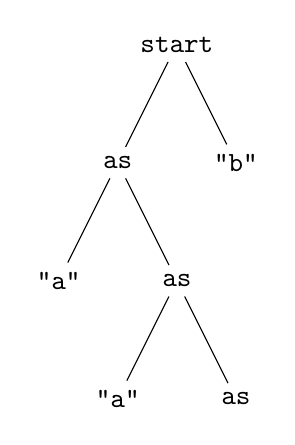
\begin{tikzpicture}
\node {\texttt{start}}
  child {node {\texttt{as}}
    child {node {\texttt{"a"}}}
    child {node {\texttt{as}}
      child {node {\texttt{"a"}}}
      child {node {\texttt{as}}}}}
  child {node {\texttt{"b"}}};
\end{tikzpicture}
\caption{\textit{Parse tree} graph for \texttt{aab}}
\end{subfigure}
\caption{Example of a CFG and its \textit{parse tree}}
\label{fig:cfg_parse_tree_example}
\end{figure}

\subsection{Answer Set Grammars}

ASGs are an extension of CFGs, whereby each production rule is \textit{annotated}. More specifically, $P$ can be a \textit{ground term}, such as in the \textit{annotated atom} \texttt{a(1)@2} (referring to the second child of this node). The example shown in Figure \ref{fig:asg_example} is a subset of the language \texttt{a\textsuperscript{i}b} captured by the CFG in Figure \ref{fig:cfg_parse_tree_example},  restricting it to the language \texttt{a\textsuperscript{n}} where $\texttt{n} \ge 2$ (the string contains at least two as).

\begin{definition}[Answer Set Grammar \cite{law_representing_2019}]
 An \textit{annotated} production rule is of the form $n_0 \to n_1 ... n_k\ P$ where $n_0 \to n_1 ... n_k$ is an ordinary CFG production rule and $P$ is an \textit{annotated} ASP program, where every \textit{annotation} is an integer from $1$ to $k$.
\end{definition}

\begin{figure}[H]
\texttt{1: start -> as "b" \{ :- size(X)@1, X < 1. \} \\
           2: as -> "a" as \space\space\space\{ size(X+1) :- size(X)@2. \} \\
           3: as -> \space\space\space\space\space\space\space\space\space\space\{ size(0). \} \\}\\
* Intuitively, \texttt{size} represents the length of the current string.
\caption{Example of an ASG}
\label{fig:asg_example}
\end{figure}

\begin{definition}[Parse Tree Program \cite{law_representing_2019}]
Let G be an ASG and PT be a \textit{parse tree}. $G[PT]$ is the program $\{\ rule(n)@trace(n)\ |\ n \in PT\ \}$, where for any production rule $n_0 \to n_1...n_k\ P$, and any trace $t$, $PR@t$ is the program constructed by replacing all annotated atoms $a@i$ with the atom $a@t++[i]$ and all \textit{unannotated atoms} $a$ with the atom $a@t$.
\end{definition}

\begin{definition}[Conforming Parse Tree \cite{law_representing_2019}]
Given a string $str$ of terminal nodes, we say that $str \in \mathcal{L}(G)$ ($str$ \textit{conforms} to the language of G) if and only if there exists a parse tree PT of G for $str$ such that the program $G[PT]$ is \textit{satisfiable}. For such a PT, every single rule in the language must be satisfied (see Definition \ref{def:satisfiability}).
\end{definition}

As shown in Figure \ref{fig:asg_tree_program_example}, $\texttt{aab} \in \mathcal{L}(G)$, and the corresponding program has a single answer set $\{size(0)@[1,2,2],\ size(1)@[1,2],\ size(2)@[1]\}$. From this example, it is easy to see how the corresponding program would be \textit{unsatisfiable} for the string \texttt{ab}.

\begin{figure}[H]
\centering
\texttt{:- size(X)@[1], X < 1. \\
           size(X+1)@[1] :- size(X)@[1,2]. \\
           size(X+1)@[1,2] :- size(X)@[1,2,2]. \\
           size(0)@[1,2,2].}
\caption{$G[PT]$ for the \textit{parse tree} and ASG from the examples above}
\label{fig:asg_tree_program_example}
\end{figure}

\subsection{Learning Answer Set Grammars}

Given an incomplete ASG, it is possible to learn the complete grammar by induction (which uses \href{http://www.ilasp.com}{ILASP}), as long as we provide some \textit{positive examples} (strings which should conform to the language) and/or \textit{negative examples}  (strings which must not), as well as a \textit{hypothesis space} and usually some \textit{background} information. Note that the \textit{background} is only used for ``global" knowledge, such as defining what is a number, or how to increment one \cite{law_representing_2019}.

In such an \textit{inductive learning program} (ILP) task, we have a \textit{hypothesis space} in the form of \textit{mode declarations}, defining the format of the heads (written \texttt{\#modeh}) and bodies (written \texttt{\#modeb}) of rules which can be learned. It is also possible to restrict the scope of a particular \textit{mode declaration} by specifying a list of rule numbers at the end. Note that there are two forms of body \textit{mode declarations}: \texttt{\#modeba} is used for predicates that accept an $@$ \textit{annotation}, and \texttt{\#modebb} is intended for those without (which are defined in \texttt{\#background}). An example is shown in Figure \ref{fig:asg_ilp_example}.

\begin{figure}[H]
\centering
\begin{subfigure}{0.55\textwidth}
\texttt{start -> as bs \{\} \\
as -> "a" as \{\} | \{\} \\
bs -> "b" bs \{\} | \{\} \\
\newline
+ [] \\
+ ["a", "b"] \\
+ ["a", "a", "b", "b"] \\
- ["a"] \\
- ["b"] \\
- ["a", "a"] \\
- ["b", "b"] \\
- ["a", "a", "b"] \\
- ["a", "b", "b"] \\
\newline
\#background \{ \\
num(0). num(1). num(2). num(3). \\
inc(X,X+1) :- num(X), num(X+1). \} \\
\newline
\#modeh(size(var(num))):[2,3,4,5]. \\
\#modeh(size(0)):[2,3,4,5]. \\
\#modeba(size(var(num))). \\}
\caption{Input incomplete program}
\end{subfigure}
\begin{subfigure}{0.44\textwidth}
\texttt{start -> as bs \{ \\
\phantom{ }:- not size(X)@2, size(X)@1. \\
\} \\
\newline
as -> "a" as \{ \\
\phantom{ }size(X+1) :- size(X)@2. \\
\} \\
\newline
as -> \{ \\
\phantom{ }size(0). \\
\} \\
\newline
bs -> "b" bs \{ \\
\phantom{ }size(X+1) :- size(X)@2. \\
\} \\
\newline
bs -> \{ \\
\phantom{ }size(0). \\
\}} \\
\caption{Output learned program}
\end{subfigure}
\newline
\newline
* Note: the symbol \texttt{|} indicates multiplicity of production rules.
\caption{Example of an ASG ILP task for the language \texttt{a\textsuperscript{n}b\textsuperscript{n}}}
\label{fig:asg_ilp_example}
\end{figure}

\section{Neural Networks}

\subsection{Recurrent Neural Networks}

A recurrent neural network (RNN) is a chain-like neural network that is applied once for each \textit{token} in the input sequence. At each timestep $t$ in a ``vanilla" RNN (i.e., for each item in the sequence), the current \textit{hidden state} $h_t$ is computed as a function of the previous \textit{hidden state} $h_{t-1}$ and the current input \textit{token} $x_t$, using a non-linear \textit{activation function} (usually sigmoid) \cite{cho_learning_2014}.

\subsection{Long Short-Term Memories}

A long short-term memory (LSTM) is a particular kind of RNN, motivated by the problems of vanishing and exploding gradients which sometimes occur due to the chain-like nature of RNNs. The solution here is to at each timestep use what is called a \textit{memory block}, which holds at it center a linear unit that is connected to itself. In addition, it has three \textit{gates}: input ($i$), forget ($f$) and output ($o$). Respectively, these three \textit{gates} are concerned with which information to store, how long to store it, and when it should be passed on \cite{gers_learning_2000}.

Finally, each \textit{memory block} also stores a \textit{cell state} $c_t$, which combines information from the previous \textit{cell state} $c_{t-1}$ and from the \textit{candidate state} $g_t$ (defined as per the \textit{hidden state} in a vanilla RNN), using the \textit{forget} and \textit{input} \textit{gates} to regulate information flow. The \textit{hidden state} $h_t$ is then defined as a function of this \textit{cell state}, controlled by the \textit{output gate}. Figure \ref{fig:memory_block} shows this diagrammatically \cite{graves_hybrid_2013}.

\begin{equation}
\begin{aligned}
i_t &= \sigma(W_{xi} \cdot x_t + W_{hi} \cdot h_{t-1} + W_{ci} \cdot c_{t-1} + b_i) \\
f_t &= \sigma(W_{xf} \cdot x_t + W_{hf} \cdot h_{t-1} + W_{cf} \cdot c_{t-1} + b_f) \\
o_t &= \sigma(W_{xo} \cdot x_t + W_{ho} \cdot h_{t-1} + W_{co} \cdot c_t + b_o) \\
g_t &= tanh(W_{xg} \cdot x_t + W_{hg} \cdot h_{t-1} + b_g) \\
c_t &= f_t \cdot c_{t-1} + i_t \cdot g_t \\
h_t &= tanh(c_t)
\end{aligned}
\end{equation}

\begin{figure}[H]
\centering
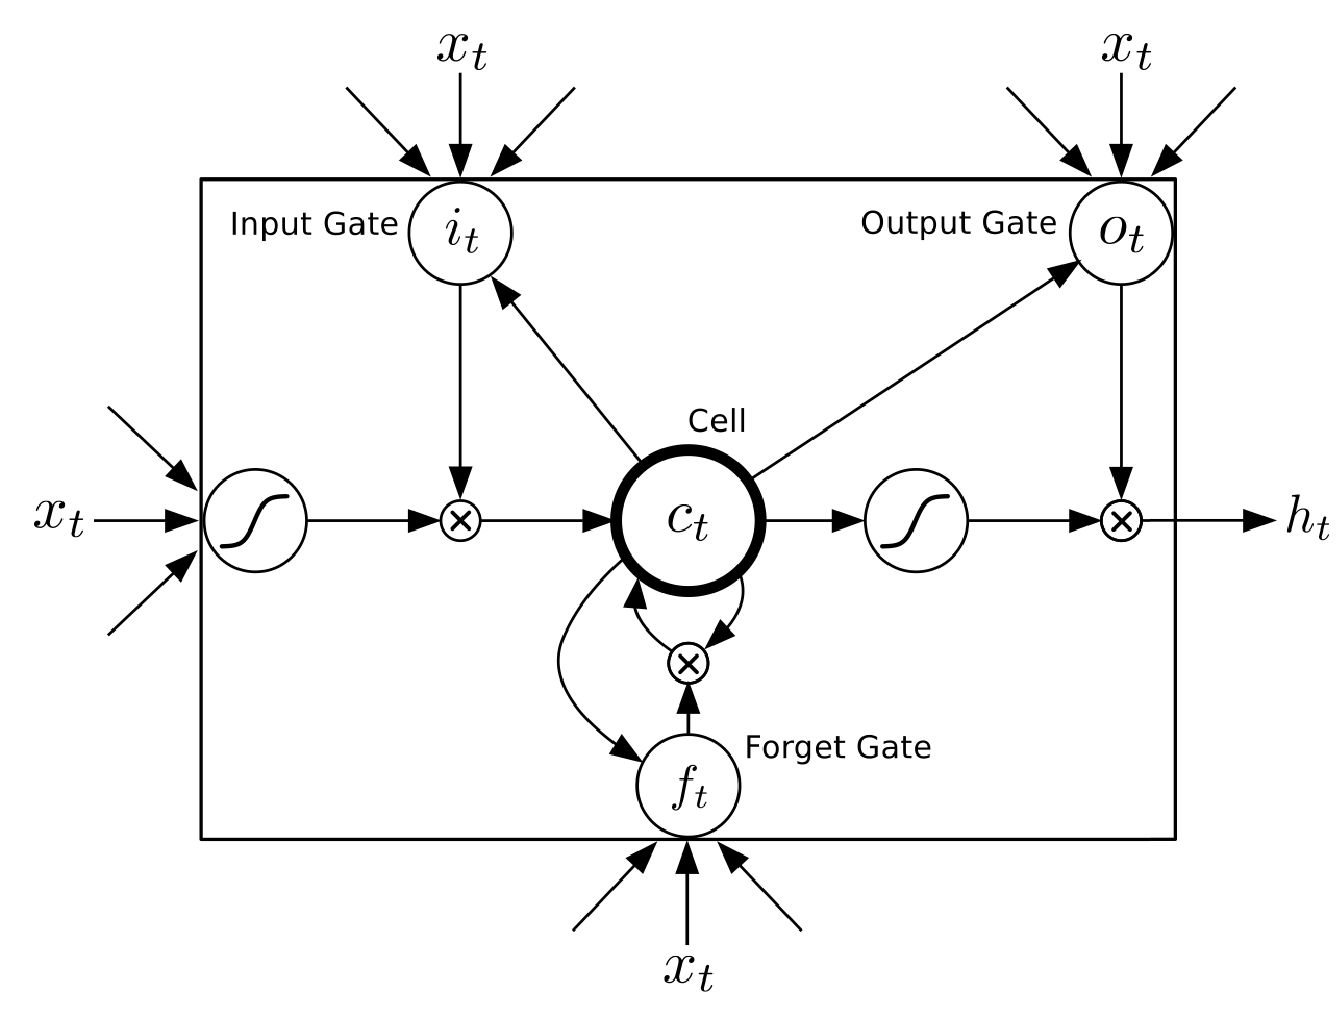
\includegraphics[width=0.62\textwidth]{memory_block.eps}
\caption{\cite{graves_hybrid_2013} Diagram showing the flow of information in an LSTM \textit{memory block}}
\label{fig:memory_block}
\end{figure}

\subsection{Encoder-Decoders}

An \textit{encoder-decoder} is a neural network consisting of two eponymous RNNs, are often LSTMs. The \textit{encoder}'s job is to translate any variable-length sequence given as input into a fixed-length vector representation, while the \textit{decoder}'s role is to transform this into a new variable-length sequence. Together, they are trained to maximize the probability of generating a target sequence given the corresponding input sequence \cite{cho_learning_2014}.

\subsection{Attention}

In the context of neural machine translation (NMT) systems such as \textit{encoder-decoders}, the driver behind \textit{attention} is to improve performance by selectively looking at sub-portions of the input sequence, which becomes especially important for long sequences of text \cite{yao_dual_2018}.

\subsubsection{Global Attention}

On top of being dependant on the last \textit{hidden state} $d_{t-1}$ and output \textit{token} $y_{i-1}$, every \textit{hidden state} $d_t$ in a \textit{decoder} with \textit{global attention} is computed also in function of its \textit{context vector} $c_t$. Each \textit{context vector} $c_t$ is defined as a weighted sum of the \textit{encoder}'s \textit{hidden states} $h_i$. The $h_i$ that are assigned a higher weight are that which are more similar to $d_t$, which is done using a trainable \textit{alignment model} $a$ \cite{bahdanau_neural_2016}.

\begin{equation}
\begin{aligned}
c_t &= \sum_{i} \alpha_{ti} \cdot h_t \\
\mbox{where } \alpha_{ti} &= \frac{exp(s_{ti})}{\sum_{j} exp(s_{tj})} \\
s_{ti} &= a(d_{t-1},h_i)
\end{aligned}
\end{equation}

Here the idea is that $\alpha_{ti}$ tells us how important each $h_i$ is with respect to the current timestep $t$, influencing the value of $d_t$ and hence the decision of the generated output \textit{token} $y_t$. Essentially, this is a way of telling the \textit{decoder} which parts of the input sequence to pay attention to. Thanks to this mechanism, the \textit{encoder} is no longer forced to compress all the useful information from an input sequence into a fixed-length vector, thus improving performance for longer sequences of \textit{tokens} \cite{bahdanau_neural_2016}.

\chapter{Preprocessor}
\section{Overview}

In order to... as shown in Figure \ref{fig:preprocessor_pipeline}.

\begin{figure}[H]
\centering

\begin{tikzpicture}[node distance=0.55cm, auto]
\node (story_in) [] {Story};
\node (tokenize) [block, right =of story_in] {Tokenize};
\node (simplify) [block, right =of tokenize] {Simplify};
\node (prune) [block, right =of simplify] {Prune};
\node (homogenise) [block, right =of prune] {Homogenise};
\node (story_out) [block, right =of homogenise] {Preprocessed Story};
\draw [->] (story_in) -- (tokenize);
\draw [->] (tokenize) -- (simplify);
\draw [->] (simplify) -- (prune);
\draw [->] (prune) -- (homogenise);
\draw [->] (homogenise) -- (story_out);
\end{tikzpicture}
\caption{Preprocessor Steps}
\label{fig:preprocessor_pipeline}
\end{figure}

\section{Tokenization and Simplification}

\section{Sentence Pruning and Homogenisation}

\section{Expandability}

\textcolor{red}{\textbf{\hl{TODO}}}

\chapter{ASG}
\label{appendix:asg}

\chapter{ASG}

Although \textsc{SumASG\textsubscript{1}} and \textsc{SumASG\textsubscript{2}} share the same grammar, they need to augment a few of its derivations with some extra rules. The code that you see in Sections \ref{sec:appendix_asg_1} and \ref{sec:appendix_asg_2} gets appended to the general grammar, giving the complete ASG program.

\section{Common Grammar}

\begin{lstlisting}
start -> s_group {
   :- count(X)@1, X > 1.
   :- count(X)@1, X = 0.
}

s_group -> {
  count(0).
}

s_group -> s_group s ``. " {
  count(X+1) :- count(X)@1.

  % Reject output summaries with duplicate sentences
  sentence(X,V,O,S) :- output(_,V,O,S)@2, count(X).
  sentence(X,V,O,S) :- sentence(X,V,O,S)@1.
  :- sentence(X1,V,O,S), sentence(X2,V,O,S), X1 != X2.
}

s -> np vp {
  subject :- subject(S_N,S_D,S_A)@1.
  :- not subject.
  object :- object(S_N,S_D,S_A)@2.
  :- not object.
}

vp -> vbn np {
  verb(N,T) :- verb(N,T)@1.
  object(N,D,A) :- object(N,D,A)@2.
}

vp -> vbd np {
  verb(N,T) :- verb(N,T)@1.
  object(N,D,A) :- object(N,D,A)@2.
}

vp -> vbd vbg np {
  verb(comp(N1,N2),comp(T1,gerund)) :- verb(N1,T1)@1, verb(N2,gerund)@2.
  object(N,D,A) :- object(N,D,A)@3.
}

vp -> vbd vbn np {
  verb(comp(N1,N2),comp(T1,past_part)) :- verb(N1,T1)@1, verb(N2,past_part)@2.
  object(N,D,A) :- object(N,D,A)@3.
}

vp -> vbd ``to " vb np {
  verb(comp(N1,N2),comp(T1,base)) :- verb(N1,T1)@1, verb(N2,base)@3.
  object(N,D,A) :- object(N,D,A)@4.
}

vp -> vbp np {
  verb(N,T) :- verb(N,T)@1.
  object(N,D,A) :- object(N,D,A)@2.
}

vp -> vbp vbg np {
  verb(comp(N1,N2),comp(T1,gerund)) :- verb(N1,T1)@1, verb(N2,gerund)@2.
  object(N,D,A) :- object(N,D,A)@3.
}

vp -> vbp vbn np {
  verb(comp(N1,N2),comp(T1,past_part)) :- verb(N1,T1)@1, verb(N2,past_part)@2.
  object(N,D,A) :- object(N,D,A)@3.
}

vp -> vbp ``to " vb np {
  verb(comp(N1,N2),comp(T1,base)) :- verb(N1,T1)@1, verb(N2,base)@3.
  object(N,D,A) :- object(N,D,A)@4.
}

vp -> vbz np {
  verb(N,T) :- verb(N,T)@1.
  object(N,D,A) :- object(N,D,A)@2.
}

vp -> vbz vbg np {
  verb(comp(N1,N2),comp(T1,gerund)) :- verb(N1,T1)@1, verb(N2,gerund)@2.
  object(N,D,A) :- object(N,D,A)@3.
}

vp -> vbz vbn np {
  verb(comp(N1,N2),comp(T1,past_part)) :- verb(N1,T1)@1, verb(N2,past_part)@2.
  object(N,D,A) :- object(N,D,A)@3.
}

vp -> vbz ``to " vb np {
  verb(comp(N1,N2),comp(T1,base)) :- verb(N1,T1)@1, verb(N2,base)@3.
  object(N,D,A) :- object(N,D,A)@4.
}

np -> np rb {
  object(N,D,A) :- object(N,D,0)@1, adj_or_adv(A)@2.
}

np -> np rb {
  object(N,D,conjunct(A1,A2)) :- object(N,D,A1)@1, adj_or_adv(A2)@2.
  :- object(N,D,conjunct(A,A)).
}

np -> np rp {
  object(N,D,A) :- object(N,D,0)@1, adj_or_adv(A)@2.
}

np -> np rp {
  object(N,D,conjunct(A1,A2)) :- object(N,D,A1)@1, adj_or_adv(A2)@2.
  :- object(N,D,conjunct(A,A)).
}

np -> nn {
  subject(N,0,0) :- noun(N)@1.
  object(N,0,0) :- noun(N)@1.
}

np -> nns {
  subject(N,0,0) :- noun(N)@1.
  object(N,0,0) :- noun(N)@1.
}

np -> nnp {
  subject(N,0,0) :- noun(N)@1.
  object(N,0,0) :- noun(N)@1.
}

np -> nnps {
  subject(N,0,0) :- noun(N)@1.
  object(N,0,0) :- noun(N)@1.
}

np -> prp {
  subject(N,0,0) :- noun(N)@1.
  object(N,0,0) :- noun(N)@1.
}

np -> rb {
  subject(0,0,A) :- adj_or_adv(A)@1.
  object(0,0,A) :- adj_or_adv(A)@1.
}

np -> rp {
  subject(0,0,A) :- adj_or_adv(A)@1.
  object(0,0,A) :- adj_or_adv(A)@1.
}

np -> ex {
  subject(N,0,0) :- noun(N)@1.
}

np -> in {
  object(0,D,0) :- det(D)@1.
}

np -> prp ``and " nnp {
  subject(conjunct(N1,N2),0,0) :- noun(N1)@1, noun(N2)@3.
  object(conjunct(N1,N2),0,0) :- noun(N1)@1, noun(N2)@3.
  :- subject(conjunct(N,N),0,0).
  :- object(conjunct(N,N),0,0).
}

np -> nnp ``and " prp {
  subject(conjunct(N1,N2),0,0) :- noun(N1)@1, noun(N2)@3.
  object(conjunct(N1,N2),0,0) :- noun(N1)@1, noun(N2)@3.
  :- subject(conjunct(N,N),0,0).
  :- object(conjunct(N,N),0,0).
}

np -> dt nn ``and " prp {
  subject(conjunct(N1,N2),D,0) :- det(D)@1, noun(N1)@2, noun(N2)@4.
  object(conjunct(N1,N2),D,0) :- det(D)@1, noun(N1)@2, noun(N2)@4.
  :- subject(conjunct(N,N),_,0).
  :- object(conjunct(N,N),_,0).
}

np -> prp ``and " dt nn {
  subject(conjunct(N1,N2),D,0) :- noun(N1)@1, det(D)@3, noun(N2)@4.
  object(conjunct(N1,N2),D,0) :- noun(N1)@1, det(D)@3, noun(N2)@4.
  :- subject(conjunct(N,N),_,0).
  :- object(conjunct(N,N),_,0).
}

np -> dt nn ``and " nnp {
  subject(conjunct(N1,N2),D,0) :- det(D)@1, noun(N1)@2, noun(N2)@4.
  object(conjunct(N1,N2),D,0) :- det(D)@1, noun(N1)@2, noun(N2)@4.
  :- subject(conjunct(N,N),_,0).
  :- object(conjunct(N,N),_,0).
}

np -> nnp ``and " dt nn {
  subject(conjunct(N1,N2),D,0) :- noun(N1)@1, det(D)@3, noun(N2)@4.
  object(conjunct(N1,N2),D,0) :- noun(N1)@1, det(D)@3, noun(N2)@4.
  :- subject(conjunct(N,N),_,0).
  :- object(conjunct(N,N),_,0).
}

np -> nnp ``and " nnp {
  subject(conjunct(N1,N2),0,0) :- noun(N1)@1, noun(N2)@3.
  object(conjunct(N1,N2),0,0) :- noun(N1)@1, noun(N2)@3.
  :- subject(conjunct(N,N),0,0).
  :- object(conjunct(N,N),0,0).
}

np -> nn ``and " nn {
  subject(conjunct(N1,N2),0,0) :- noun(N1)@1, noun(N2)@3.
  object(conjunct(N1,N2),0,0) :- noun(N1)@1, noun(N2)@3.
  :- subject(conjunct(N,N),0,0).
  :- object(conjunct(N,N),0,0).
}

np -> nn ``and " nns {
  subject(conjunct(N1,N2),0,0) :- noun(N1)@1, noun(N2)@3.
  object(conjunct(N1,N2),0,0) :- noun(N1)@1, noun(N2)@3.
  :- subject(conjunct(N,N),0,0).
  :- object(conjunct(N,N),0,0).
}

np -> nns ``and " nn {
  subject(conjunct(N1,N2),0,0) :- noun(N1)@1, noun(N2)@3.
  object(conjunct(N1,N2),0,0) :- noun(N1)@1, noun(N2)@3.
  :- subject(conjunct(N,N),0,0).
  :- object(conjunct(N,N),0,0).
}

np -> nns ``and " nns {
  subject(conjunct(N1,N2),0,0) :- noun(N1)@1, noun(N2)@3.
  object(conjunct(N1,N2),0,0) :- noun(N1)@1, noun(N2)@3.
  :- subject(conjunct(N,N),0,0).
  :- object(conjunct(N,N),0,0).
}

np -> dt nn ``and " dt nn {
  subject(conjunct(N1,N2),D,0) :- det(D)@1, det(D)@4, noun(N1)@2, noun(N2)@5.
  object(conjunct(N1,N2),D,0) :- det(D)@1, det(D)@4, noun(N1)@2, noun(N2)@5.
  :- subject(conjunct(N,N),_,0).
  :- object(conjunct(N,N),_,0).
}

np -> prp ``and " prp {
  subject(conjunct(N1,N2),0,0) :- noun(N1)@1, noun(N2)@3.
  object(conjunct(N1,N2),0,0) :- noun(N1)@1, noun(N2)@3.
  :- subject(conjunct(N,N),0,0).
  :- object(conjunct(N,N),0,0).
}

np -> rb ``and " rb {
  subject(0,0,conjunct(A1,A2)) :- adj_or_adv(A1)@1, adj_or_adv(A2)@3.
  object(0,0,conjunct(A1,A2)) :- adj_or_adv(A1)@1, adj_or_adv(A2)@3.
  :- subject(0,0,conjunct(A,A)).
  :- object(0,0,conjunct(A,A)).
}

np -> jj {
  object(0,0,A) :- adj_or_adv(A)@1.
}

np -> jj ``and " jj {
  object(0,0,conjunct(A1,A2)) :- adj_or_adv(A1)@1, adj_or_adv(A2)@3.
  :- object(0,0,conjunct(A,A)).
}

np -> jj rb {
  subject(0,0,conjunct(A1,A2)) :- adj_or_adv(A1)@1, adj_or_adv(A2)@1.
  object(0,0,conjunct(A1,A2)) :- adj_or_adv(A1)@1, adj_or_adv(A2)@1.
  :- subject(0,0,conjunct(A,A)).
  :- object(0,0,conjunct(A,A)).
}

np -> dt nn {
  subject(N,D,0) :- det(D)@1, noun(N)@2.
  object(N,D,0) :- det(D)@1, noun(N)@2.
}

np -> dt nns {
  subject(N,D,0) :- det(D)@1, noun(N)@2.
  object(N,D,0) :- det(D)@1, noun(N)@2.
}

np -> jj nns {
  subject(N,0,A) :- adj_or_adv(A)@1, noun(N)@2.
  object(N,0,A) :- adj_or_adv(A)@1, noun(N)@2.
}

np -> jj nnp {
  subject(N,0,A) :- adj_or_adv(A)@1, noun(N)@2.
  object(N,0,A) :- adj_or_adv(A)@1, noun(N)@2.
}

np -> jj nnps {
  subject(N,0,A) :- adj_or_adv(A)@1, noun(N)@2.
  object(N,0,A) :- adj_or_adv(A)@1, noun(N)@2.
}

np -> dt jj nn {
  subject(N,D,A) :- det(D)@1, adj_or_adv(A)@2, noun(N)@3.
  object(N,D,A) :- det(D)@1, adj_or_adv(A)@2, noun(N)@3.
}

np -> dt jj nns {
  subject(N,D,A) :- det(D)@1, adj_or_adv(A)@2, noun(N)@3.
  object(N,D,A) :- det(D)@1, adj_or_adv(A)@2, noun(N)@3.
}

np -> dt jj jj nn {
  subject(N,D,conjunct(A1,A2)) :- det(D)@1, adj_or_adv(A1)@2, adj_or_adv(A2)@3, noun(N)@4.
  object(N,D,conjunct(A1,A2)) :- det(D)@1, adj_or_adv(A1)@2, adj_or_adv(A2)@3, noun(N)@4.
  :- subject(N,D,conjunct(A,A)).
  :- object(N,D,conjunct(A,A)).
}

np -> dt jj jj nns {
  subject(N,D,conjunct(A1,A2)) :- det(D)@1, adj_or_adv(A1)@2, adj_or_adv(A2)@3, noun(N)@4.
  object(N,D,conjunct(A1,A2)) :- det(D)@1, adj_or_adv(A1)@2, adj_or_adv(A2)@3, noun(N)@4.
  :- subject(N,D,conjunct(A,A)).
  :- object(N,D,conjunct(A,A)).
}

np -> dt jjr nn {
  subject(N,D,A) :- det(D)@1, adj_or_adv(A)@2, noun(N)@3.
  object(N,D,A) :- det(D)@1, adj_or_adv(A)@2, noun(N)@3.
}

np -> dt jjr nns {
  subject(N,D,A) :- det(D)@1, adj_or_adv(A)@2, noun(N)@3.
  object(N,D,A) :- det(D)@1, adj_or_adv(A)@2, noun(N)@3.
}

np -> dt jjs nn {
  subject(N,D,A) :- det(D)@1, adj_or_adv(A)@2, noun(N)@3.
  object(N,D,A) :- det(D)@1, adj_or_adv(A)@2, noun(N)@3.
}

np -> dt jjs nns {
  subject(N,D,A) :- det(D)@1, adj_or_adv(A)@2, noun(N)@3.
  object(N,D,A) :- det(D)@1, adj_or_adv(A)@2, noun(N)@3.
}

np -> in nn {
  object(N,D,0) :- det(D)@1, noun(N)@2.
}

np -> in dt nn {
  object(N,conjunct(D1,D2),0) :- det(D1)@1, det(D2)@2, noun(N)@3.
}

np -> in nns {
  object(N,D,0) :- det(D)@1, noun(N)@2.
}

np -> in dt nns {
  object(N,conjunct(D1,D2),0) :- det(D1)@1, det(D2)@2, noun(N)@3.
}

np -> in nnp {
  object(N,D,0) :- det(D)@1, noun(N)@2.
}

np -> in nnps {
  object(N,D,0) :- det(D)@1, noun(N)@2.
}

np -> jj in nn {
  object(N,D,A) :- adj_or_adv(A)@1, det(D)@2, noun(N)@3.
}

np -> jj in nn ``and " nn {
  object(conjunct(N1,N2),D,A) :- adj_or_adv(A)@1, det(D)@2, noun(N1)@3, noun(N2)@5.
}

np -> jj in nns {
  object(N,D,A) :- adj_or_adv(A)@1, det(D)@2, noun(N)@3.
}

np -> jj in nns ``and " nns {
  object(conjunct(N1,N2),D,A) :- adj_or_adv(A)@1, det(D)@2, noun(N1)@3, noun(N2)@5.
}

np -> jj in nnp {
  object(N,D,A) :- adj_or_adv(A)@1, det(D)@2, noun(N)@3.
}

np -> jj in nnp ``and " nnp {
  object(conjunct(N1,N2),D,A) :- adj_or_adv(A)@1, det(D)@2, noun(N1)@3, noun(N2)@5.
}

np -> jj in prp {
  object(N,D,A) :- adj_or_adv(A)@1, det(D)@2, noun(N)@3.
}

np -> jj in prp ``and " prp {
  object(conjunct(N1,N2),D,A) :- adj_or_adv(A)@1, det(D)@2, noun(N1)@3, noun(N2)@5.
}

np -> jj in nn ``and " nns {
  object(conjunct(N1,N2),D,A) :- adj_or_adv(A)@1, det(D)@2, noun(N1)@3, noun(N2)@5.
}

np -> jj in nns ``and " nn {
  object(conjunct(N1,N2),D,A) :- adj_or_adv(A)@1, det(D)@2, noun(N1)@3, noun(N2)@5.
}

np -> cd nn {
  subject(N,D,0) :- det(D)@1, noun(N)@2.
  object(N,D,0) :- det(D)@1, noun(N)@2.
}

np -> cd nns {
  subject(N,D,0) :- det(D)@1, noun(N)@2.
  object(N,D,0) :- det(D)@1, noun(N)@2.
}

np -> cd jj nn {
  subject(N,D,A) :- det(D)@1, adj_or_adv(A)@2, noun(N)@3.
  object(N,D,A) :- det(D)@1, adj_or_adv(A)@2, noun(N)@3.
}

np -> cd jj nns {
  subject(N,D,A) :- det(D)@1, adj_or_adv(A)@2, noun(N)@3.
  object(N,D,A) :- det(D)@1, adj_or_adv(A)@2, noun(N)@3.
}

np -> cd nns jj {
  object(N,D,A) :- det(D)@1, noun(N)@2, adj_or_adv(A)@3.
}

np -> dt jj cd {
  subject(0,conjunct(D1,D2),A) :- det(D1)@1, adj_or_adv(A)@2, det(D2)@3.
  object(0,conjunct(D1,D2),A) :- det(D1)@1, adj_or_adv(A)@2, det(D2)@3.
}
\end{lstlisting}

\vspace{5pt}

\section{Task: \textsc{SumASG\textsubscript{1}}}
\label{sec:appendix_asg_1}

\begin{lstlisting}
s -> np vp {
  ...
  
  :- not action(verb(V_N,V_T),subject(S_N,S_D,S_A),object(O_N,O_D,O_A)), verb(V_N,V_T)@2, subject(S_N,S_D,S_A)@1, object(O_N,O_D,O_A)@2.
}

#modeh(action(verb(const(main_verb),const(main_form)), subject(const(noun),const(det),const(adj_or_adv)), object(const(noun),const(det),const(adj_or_adv)))):[4].
#modeh(action(verb(const(main_verb),const(main_form)), subject(const(noun),const(det),const(adj_or_adv)), object(const(noun),const(det),conjunct(const(adj_or_adv),const(adj_or_adv))))):[4].
#modeh(action(verb(const(main_verb),const(main_form)), subject(const(noun),const(det),conjunct(const(adj_or_adv),const(adj_or_adv))), object(const(noun),const(det),const(adj_or_adv)))):[4].
#modeh(action(verb(const(main_verb),const(main_form)), subject(conjunct(const(noun),const(noun)),const(det),const(adj_or_adv)), object(const(noun),const(det),const(adj_or_adv)))):[4].
#modeh(action(verb(const(main_verb),const(main_form)), subject(const(noun),const(det),const(adj_or_adv)), object(conjunct(const(noun),const(noun)),const(det),const(adj_or_adv)))):[4].
#modeh(action(verb(const(main_verb),const(main_form)), subject(const(noun),const(det),const(adj_or_adv)), object(const(noun),conjunct(const(det),const(det)),const(adj_or_adv)))):[4].
#modeh(action(verb(const(main_verb),const(main_form)), subject(const(noun),const(det),const(adj_or_adv)), object(const(noun),conjunct(const(prep),const(det)),const(adj_or_adv)))):[4].

#modeh(action(verb(comp(const(main_verb),const(aux_verb)),comp(const(main_form),const(aux_form))), subject(const(noun),const(det),const(adj_or_adv)), object(const(noun),const(det),const(adj_or_adv)))):[4].
#modeh(action(verb(comp(const(main_verb),const(aux_verb)),comp(const(main_form),const(aux_form))), subject(const(noun),const(det),const(adj_or_adv)), object(const(noun),const(det),conjunct(const(adj_or_adv),const(adj_or_adv))))):[4].
#modeh(action(verb(comp(const(main_verb),const(aux_verb)),comp(const(main_form),const(aux_form))), subject(const(noun),const(det),conjunct(const(adj_or_adv),const(adj_or_adv))), object(const(noun),const(det),const(adj_or_adv)))):[4].
#modeh(action(verb(comp(const(main_verb),const(aux_verb)),comp(const(main_form),const(aux_form))), subject(conjunct(const(noun),const(noun)),const(det),const(adj_or_adv)), object(const(noun),const(det),const(adj_or_adv)))):[4].

#bias(":- head(holds_at_node(action(verb(_,_),subject(0,_,_),object(_,_,_)),var__(1))).").
#bias(":- head(holds_at_node(action(verb(_,_),subject(_,_,_),object(0,0,0)),var__(1))).").

#bias(":- head(holds_at_node(action(verb(_,_),subject(_,_,_),object(conjunct(V,V),_,_)),var__(1))).").
#bias(":- head(holds_at_node(action(verb(_,_),subject(_,_,_),object(conjunct(_,0),_,_)),var__(1))).").
#bias(":- head(holds_at_node(action(verb(_,_),subject(_,_,_),object(conjunct(0,_),_,_)),var__(1))).").

#bias(":- head(holds_at_node(action(verb(_,_),subject(_,_,_),object(_,_,conjunct(V,V))),var__(1))).").
#bias(":- head(holds_at_node(action(verb(_,_),subject(_,_,_),object(_,_,conjunct(_,0))),var__(1))).").
#bias(":- head(holds_at_node(action(verb(_,_),subject(_,_,_),object(_,_,conjunct(0,_))),var__(1))).").

#bias(":- head(holds_at_node(action(verb(_,_),subject(conjunct(V,V),_,_),object(_,_,_)),var__(1))).").
#bias(":- head(holds_at_node(action(verb(_,_),subject(conjunct(_,0),_,_),object(_,_,_)),var__(1))).").
#bias(":- head(holds_at_node(action(verb(_,_),subject(conjunct(0,_),_,_),object(_,_,_)),var__(1))).").

#bias(":- head(holds_at_node(action(verb(_,_),subject(_,_,conjunct(V,V)),object(_,_,_)),var__(1))).").
#bias(":- head(holds_at_node(action(verb(_,_),subject(_,_,conjunct(_,0)),object(_,_,_)),var__(1))).").
#bias(":- head(holds_at_node(action(verb(_,_),subject(_,_,conjunct(0,_)),object(_,_,_)),var__(1))).").

#bias(":- head(holds_at_node(action(verb(_,_),subject(_,_,_),object(_,conjunct(V,V),_)),var__(1))).").
#bias(":- head(holds_at_node(action(verb(_,_),subject(_,_,_),object(_,conjunct(_,0),_)),var__(1))).").
#bias(":- head(holds_at_node(action(verb(_,_),subject(_,_,_),object(_,conjunct(0,_),_)),var__(1))).").

#bias(":- head(holds_at_node(action(verb(_,_),subject(_,_,conjunct(V,_)),object(_,_,conjunct(V,_))),var__(1))).").
#bias(":- head(holds_at_node(action(verb(_,_),subject(_,_,conjunct(V,_)),object(_,_,conjunct(_,V))),var__(1))).").
#bias(":- head(holds_at_node(action(verb(_,_),subject(_,_,conjunct(_,V)),object(_,_,conjunct(V,_))),var__(1))).").
#bias(":- head(holds_at_node(action(verb(_,_),subject(_,_,conjunct(_,V)),object(_,_,conjunct(_,V))),var__(1))).").

#bias(":- head(holds_at_node(action(verb(comp(V,V),comp(_,past_part)),subject(_,_,_),object(0,0,0)),var__(1))).").

#constant(noun,0).
#constant(det,0).
#constant(adj_or_adv,0).
\end{lstlisting}

\vspace{5pt}

\section{Task: \textsc{SumASG\textsubscript{2}}}
\label{sec:appendix_asg_2}

\begin{lstlisting}
s -> np vp {
  ...

  summary(0, V, S, O) :- action(_, V, S, O).

  summary(1, verb(V,T), S, object(N2,D,A)) :- action(_, verb(V,T), S, object(N2,D,_)), action(_, verb(be,T), subject(it,_,_), object(_,_,A)).
  summary(2, verb(be,T), S, object(N,D1,conjunct(A2,A3))) :- action(_, verb(be,T), S, object(N,D1,_)), action(_, verb(be,T), subject(N,D2,A1), object(_,_,conjunct(A2,A3))).

  summary(3, V, subject(N1,0,0), object(N3,D,conjunct(A1,A2))) :- action(_, V, subject(conjunct(N1,N2),_,_), object(N3,D,A1)), action(_, V, subject(N1,_,_), object(N3,D,A2)).
  summary(4, V, S, object(0,0,conjunct(A1,A2))) :- action(I1, V, S, object(_,_,A1)), action(I2, V, S, object(_,_,A2)), A1 != A2, A1 != 0, A2 != 0, I1 < I2.

  summary(5, V, S, object(conjunct(N1,N2),D,0)) :- action(I1, V, S, object(N1,0,_)), action(I2, V, S, object(N2,D,_)), N1 != N2, N1 != 0, N2 != 0, I1 < I2.
  summary(6, V, S, object(conjunct(N1,N2),D,0)) :- action(I1, V, S, object(N1,D,_)), action(I2, V, S, object(N2,0,_)), N1 != N2, N1 != 0, N2 != 0, I1 < I2.
  summary(7, V, S, object(conjunct(N1,N2),D,0)) :- action(I1, V, S, object(N1,D,_)), action(I2, V, S, object(N2,D,_)), N1 != N2, N1 != 0, N2 != 0, I1 < I2.

  summary(8, V1, subject(N, D1, conjunct(A1, A2)), object(0, 0, A3)) :- action(_, V1, subject(N, D1, A2), object(0, 0, A3)), action(_, V2, subject(_, 0, 0), object(N, D2, A1)), A1 != A3.
  summary(9, V1, subject(N, D1, conjunct(A1, A2)), object(0, 0, A3)) :- action(_, V1, subject(N, D1, A2), object(0, 0, A3)), action(_, V2, subject(_, 0, 0), object(N, D2, conjunct(A1, _))), A1 != A3.
  summary(10, V1, subject(N, D1, conjunct(A1, A2)), object(0, 0, A3)) :- action(_, V1, subject(N, D1, A2), object(0, 0, conjunct(A3,_))), action(_, V2, subject(_, 0, 0), object(N, D2, A1)), A1 != A3.

  summary(I, V, S, object(conjunct(N1,N2),D,A)) :- summary(I, V, S, object(conjunct(conjunct(N1,N2),N3),D,A)).
  summary(I, V, S, object(conjunct(N1,N2),D,A)) :- summary(I, V, S, object(conjunct(N1,conjunct(N2,N3)),D,A)).
  summary(I, V, S, object(conjunct(N2,N3),D,A)) :- summary(I, V, S, object(conjunct(conjunct(N1,N2),N3),D,A)).
  summary(I, V, S, object(conjunct(N2,N3),D,A)) :- summary(I, V, S, object(conjunct(N1,conjunct(N2,N3)),D,A)).
  summary(I, V, S, object(conjunct(N1,N3),D,A)) :- summary(I, V, S, object(conjunct(conjunct(N1,N2),N3),D,A)).
  summary(I, V, S, object(conjunct(N1,N3),D,A)) :- summary(I, V, S, object(conjunct(N1,conjunct(N2,N3)),D,A)).

  summary(I, V, S, object(N,D,conjunct(A1,A2))) :- summary(I, V, S, object(N,D,conjunct(conjunct(A1,A2),A3))).
  summary(I, V, S, object(N,D,conjunct(A1,A2))) :- summary(I, V, S, object(N,D,conjunct(A1,conjunct(A2,A3)))).
  summary(I, V, S, object(N,D,conjunct(A2,A3))) :- summary(I, V, S, object(N,D,conjunct(conjunct(A1,A2),A3))).
  summary(I, V, S, object(N,D,conjunct(A2,A3))) :- summary(I, V, S, object(N,D,conjunct(A1,conjunct(A2,A3)))).
  summary(I, V, S, object(N,D,conjunct(A1,A3))) :- summary(I, V, S, object(N,D,conjunct(conjunct(A1,A2),A3))).
  summary(I, V, S, object(N,D,conjunct(A1,A3))) :- summary(I, V, S, object(N,D,conjunct(A1,conjunct(A2,A3)))).

  % Pick exactly one summary derivation for each sentence
  0{output(I,V,S,O)}1 :- summary(I,V,S,O).
  :- not output(_,_,_,_).

  :- output(_,verb(V_N,V_T),subject(S_N,S_D,S_A),object(O_N,O_D,O_A)), not verb(V_N,V_T)@2.
  :- output(_,verb(V_N,V_T),subject(S_N,S_D,S_A),object(O_N,O_D,O_A)), not subject(S_N,S_D,S_A)@1.
  :- output(_,verb(V_N,V_T),subject(S_N,S_D,S_A),object(O_N,O_D,O_A)), not object(O_N,O_D,O_A)@2.
}
\end{lstlisting}

\chapter{Post-Processing / Scoring}
\label{chapter:postprocessing}

\section{Overview}

Once we have obtained potential sentences from ASG to be used in a summary, we now post-process these as explained in Section \ref{sec:summary_creation}. By combining them in different ways, we are able to form summaries. From these, we will retain the highest scoring ones, according to the metric detailed in Section \ref{sec:scoring}. A diagram illustrating these steps is shown below in Figure \ref{fig:postprocess_pipeline}.

\begin{figure}[H]
\centering
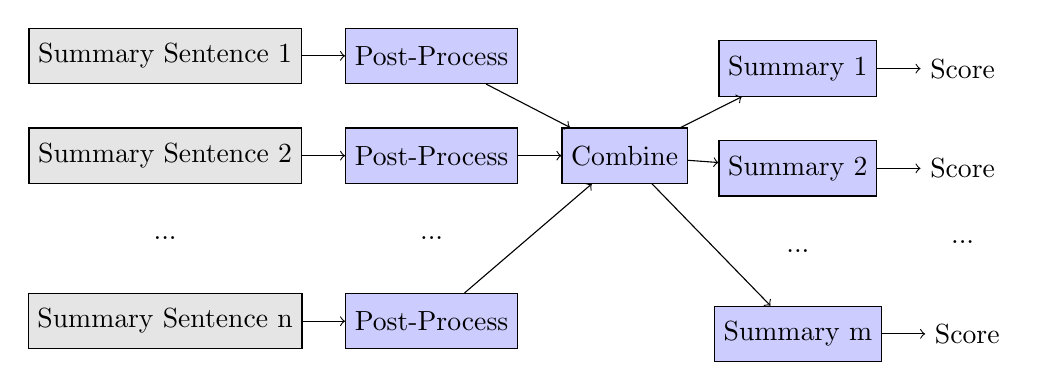
\begin{tikzpicture}[node distance=0.55cm, auto]
\node (summary_sentence_1) [inter] {Summary Sentence 1};
\node (summary_sentence_2) [inter, below =of summary_sentence_1] {Summary Sentence 2};
\node (summary_sentence_3) [below =of summary_sentence_2] {...};
\node (summary_sentence_4) [inter, below =of summary_sentence_3] {Summary Sentence n};
\node (post_process_1) [block, right =of summary_sentence_1] {Post-Process};
\node (post_process_2) [block, below =of post_process_1] {Post-Process};
\node (post_process_3) [below =of post_process_2] {...};
\node (post_process_4) [block, below =of post_process_3] {Post-Process};
\node (combine) [block, right =of post_process_2] {Combine};
\node (summary_1) [block, above right =of combine] {Summary 1};
\node (summary_2) [block, below =of summary_1] {Summary 2};
\node (summary_3) [below =of summary_2] {...};
\node (summary_4) [block, below =of summary_3] {Summary m};
\node (score_1) [right =of summary_1] {Score};
\node (score_2) [below =of score_1, right =of summary_2] {Score};
\node (score_3) [below =of score_2] {...};
\node (score_4) [below =of score_3, right =of summary_4] {Score};
\draw [->] (summary_sentence_1) -- (post_process_1);
\draw [->] (summary_sentence_2) -- (post_process_2);
\draw [->] (summary_sentence_4) -- (post_process_4);
\draw [->] (post_process_1) -- (combine);
\draw [->] (post_process_2) -- (combine);
\draw [->] (post_process_4) -- (combine);
\draw [->] (combine) -- (summary_1);
\draw [->] (combine) -- (summary_2);
\draw [->] (combine) -- (summary_4);
\draw [->] (summary_1) -- (score_1);
\draw [->] (summary_2) -- (score_2);
\draw [->] (summary_4) -- (score_4);
\end{tikzpicture}
\caption{Post-Processing / Scoring Steps}
\label{fig:postprocess_pipeline}
\end{figure}

\section{Summary Creation}
\label{sec:summary_creation}

The output of \textsc{SumASG} is a list of sentences, each of which could potentially appear in the final summary.

\subsection{Post-Processing}

\subsubsection{Grammar}

Because \textsc{SumASG} uses the same capitalization for a given word regardless of its position in the sentence, it means that the first word of each sentence will not be capitalized unless it is a proper noun. We therefore need to fix this, as well as remove the space before each full stop.

Compound nouns, whose hyphen was replaced with an underscore for the internal representation of \textsc{SumASG}, also need to be restored to their grammatically-correct form.

In addition, the task of summarization might have created a sentence where an incorrect verb form is used, or possibly the wrong determiner. To amend this we use a tool called \textbf{\href{https://pypi.org/project/language-check/}{language-check}}, which is able to correct phrases like ``they has an dog" to ``they have a dog".

\subsubsection{Complex Nouns}

One of the optimizations done by the \textsc{Preprocessor} was to combine complex nouns such as ``Peter Little" into their camel-case form ``PeterLittle", so that they would be recognized as a single \textit{token} by \textsc{SumASG}. We now need to expand them back to their original form, as this is how it should be written in English.

\subsection{Combining}

Depending on the length of the original story, we envision a different number of sentences to be in the summary, as shown below in Table \ref{tab:summary_length}.

\begin{table}[H]
\centering
\begin{tabular}{@{}llll@{}}
\toprule
Story length   & 1-2 & 3-4 & 5+ \\ \midrule
Summary length & 1   & 2   & 3  \\ \bottomrule
\end{tabular}
\caption{Length of a summary depending on the number of sentences in the story}
\label{tab:summary_length}
\end{table}

Once we have grammatically-correct summary sentences and know how many should be kept for the summary (say $n$), we generate all possible order-preserving combinations of length $n$. For instance, such combinations of length 3 for the list $[0,1,2,3]$ would be the following: $[0,1,2]$, $[0,2,3]$ and $[1,2,3]$.

\section{Scoring}
\label{sec:scoring}

Because we often end up with a large number of combinations at this phase, we need to determine which of them are best and keep only these.

\subsection{Type-Token Ratio}

To this end, we utilize an NLP metric called type-token ratio (TTR), a measure of lexical density. To provide the most informative summaries possible, we want to maximize the density of unique words.

To calculate a summary's TTR, we divide the number of unique words in the summary by the total number of words. We then divide this by number of unique words in the story and multiply it by a constant, in order to get a more consistent range for our scores.

\subsubsection{Ignored Words}

However, we do not want to neglect summaries using the same determiner, proper noun, or the verb ``to be" multiple times, as these are extremely common in English.

In addition, a story might revolve around a given \textit{topic}, which could be a person. Regarding the former, it could also be the case that the \textsc{Preprocessor} had replaced different synonyms of this \textit{topic} with a unique word.

To get around this, what we do is to exclude such words from the summary length and number of unique summary words. This way, we no longer require that these ``common" words be unique in a summary. In the following, we will call the enhanced mechanism \textsc{TTR*}.

In Figure \ref{fig:score_example} is an example which illustrates this metric. The summary with the highest final score is considered to be the best. Moreover, there is a greater difference between the summaries when using \textsc{TTR*}, which takes into account the commonly-used building blocks of the English language.

\begin{figure}[H]
\begin{subfigure}{\textwidth}
\begin{displayquote}
Jonathan was a little boy. He was hungry. Jonathan was eating an apple.
\end{displayquote}
\caption{Story}
\vspace{\baselineskip}
\end{subfigure}
\begin{subfigure}{\textwidth}
\begin{displayquote}
\textbf{A.} \underline{Jonathan} \underline{was} \underline{a} hungry boy. \underline{Jonathan} \underline{was} eating \underline{an} apple.\\
\textbf{B.} \underline{Jonathan} \underline{was} \underline{a} little boy. \underline{Jonathan} \underline{was} \underline{a} hungry boy.
\end{displayquote}
\caption{Possible summaries (underlined words will be ignored by \textsc{TTR*})}
\vspace{\baselineskip}
\end{subfigure}
\begin{subfigure}{\textwidth}
\centering
\begin{tabular}{@{}llllllll@{}}
\toprule
 & Words & Unique words & TTR & Words* & Unique words* & \textsc{TTR*} & Score \\ \midrule
\textbf{A} & 10    & 8            & 0.8 & 4      & 4             & 1    & 38    \\
\textbf{B} & 10    & 6            & 0.6 & 4      & 3             & 0.75 & 28    \\ \bottomrule
\end{tabular}
\caption{Steps for computing the score for each generated summary}
\end{subfigure}
\caption{Score computation (column headers ending with * pertain to \textsc{TTR*})}
\label{fig:score_example}
\end{figure}

\section{Summary Selection}
\label{sec:summary_selection}

\subsection{Proper Nouns}

If a story revolves around a given person and the summary mentions their name, it is preferable for this to be in the first sentence. To put this more clearly, we would like the summary of a biography to introduce the protagonist from the very first sentence. To achieve this, we simply increase the score of every summary starting with a proper noun by a constant.

\subsection{Top Summaries}

With a more complex story (5 or more sentences), it is highly likely that we will end up with a very long list of possible summaries. As there could be a number of very interesting summaries, we do not want to have to choose exactly one.

Instead, we compute 75th percentile over the scores of all generated summaries, and then discard all those whose score falls below this number. We shall call the remaining summaries \textit{top summaries}.

\subsection{Reference Summaries}

Finally, we want to be sure that our framework generates good summaries, and that the scoring works as intended. Therefore, if a story has a \textit{reference summary}, then we should make sure that there exists a similar \textit{top summary}.

In our implementation, we have chosen to use the BLEU score, which measures how closely the output given by a machine matches a text written by a human. If there exists a \textit{top summary} whose BLEU score with one of the \textit{references} is above a certain threshold, then we consider the summarization to be successful.

\section{Example}
\label{sec:postprocess_example}

An example is shown in Figure \ref{fig:postprocess_score_example} for the story of Peter Little.

The first step is to fix the grammar in the \textit{summary sentences} generated by \textsc{SumASG}, which in this case simply involves capitalizing them and removing the space before the full stop. We also need to restore the proper noun ``PeterLittle" to ``Peter Little". After \textit{combining}, we end up with 35 possible summaries.

The next step is \textit{scoring}, where we augment the standard of ignored words with the case-insensitive \textit{topics} set \{"peter", "little"\} in \textsc{TTR*}. This gives us scores in the range $[10,17]$, twenty of which fall below the 75th percentile of 15.0 and never become \textit{top summaries}.

Finally, we compare these \textit{top summaries} to our \textit{reference summaries} for Peter Little, as mentioned in Figure \ref{fig:peter_little}. At least one of them achieves a BLEU score of at least 0.65, confirming they are close enough to \textit{reference summary} \textbf{B}.

\begin{figure}[H]
\begin{subfigure}{\textwidth}
\begin{displayquote}
Peter Little is famous now.\\
The curious little boy was named Peter Little.\\
There was a curious little boy.\\
Peter Little did school always.\\
Peter Little was curious and serious.\\
Peter Little was curious in astronomy.\\
Peter Little was serious in school.
\end{displayquote}
\caption{Post-processed \textit{summary sentences}}
\end{subfigure}
\begin{subfigure}{\textwidth}
\vspace{\baselineskip}
\begin{displayquote}
\textbf{1.} Peter Little is famous now. Peter Little did school always. Peter Little was curious in astronomy.\\
\textbf{2.} Peter Little is famous now. There was a curious little boy. Peter Little did school always.\\
\textbf{3.} Peter Little is famous now. The curious little boy was named Peter Little. Peter Little did school always.\\
\textbf{4.} Peter Little is famous now. Peter Little did school always. Peter Little was curious and serious.\\
...
\end{displayquote}
\caption{\textit{Top summaries}}
\label{fig:top_score_summaries_example}
\end{subfigure}
\begin{subfigure}{\textwidth}
\vspace{\baselineskip}
\centering
\begin{tabular}{@{}lllllll@{}}
\toprule
Summary     & 1    & 2    & 3    & 4    \\ \midrule
Reference A & 0.4  & 0.38 & 0.32 & 0.38  \\
Reference B & 0.66 & 0.58 & 0.49 & 0.63 \\ \bottomrule
\end{tabular}\caption{BLEU scores for \textit{reference summaries} (summary indices as shown in Figure \ref{fig:top_score_summaries_example})}
\end{subfigure}
\caption{Example of \textit{post-processing} then \textit{scoring} for the story of Peter Little}
\label{fig:postprocess_score_example}
\end{figure}

\chapter{Possible Technical Improvements}
Had there been more time to finalise the project, there are a number of possible improvements we could have implemented. In what follows, we discuss immediate next steps which could be taken to improve each part of the pipeline.

\section{Preprocessor}

In its current state, \textsc{SumASG} expects positive sentences only, and the only form of punctuation recognized is the full stop.

\subsection{Negation}

In order to support negation, we would need to modify the structure of \textsc{SumASG}'s internal representation (see Chapter \ref{chapter:asg}). However, to achieve a better semantic understanding in \textsc{SumASG*}, we could add some more simplification logic to the \textsc{Preprocessor}.

After having implemented this, the phrase ``not happy" would be transformed into the word ``sad".

\subsection{Lists}

At the moment, \textsc{SumASG} can parse a list of length 2 at the most, i.e. a conjunction of two items. By adding a transformation to the \textsc{Preprocessor} before we modify the punctuation (see Subsection \ref{subsec:punctuation}), we could overcome this limitation. Intuitively, this would mean going from a sentence with a an $n$-item list, to $\floor{\frac{n}{2}}$ sentences with two objects and one sentence with a single object (if $n$ is odd).

For instance, the sentence ``Bob had a book, a computer and a chair." would be split into ``Bob had a book and a computer. Bob had a chair.".

\section{ASG}

Throughout the development of \textsc{SumASG}, it was a constant struggle to try and find the right balance between expressibility, summary pertinence and computational efficiency.

\subsection{Missing English Structures}

Although our general grammar allows for a wide range in terms of the words that can be used to form a sentence, to no extent does it cover even a tenth of the sentences that are used in formal or informal English. Even if you were to consider only sentences consisting of exactly one clause, \textsc{SumASG} is incapable of understanding most non-general structures commonly used in English.

By greatly simplifying the input story using the \textsc{Preprocessor}, we were able to alleviate a large part of this struggle. However if we were to use our general grammar for a task other than summarization, we would most likely run into issues due to loss of information.

\subsection{Missing Summarization Rules}

In its current implementation, \textsc{SumASG\textsubscript{2}} only uses 12 summary generation rules, one of which simply repeats the given \textit{action}. While this is largely sufficient to demonstrate the potential of our approach, in no way can it be used as is in a production text summarization tool.

In order to augment this suite of rules, it would be simple to define a \textit{mode bias} to learn summary generation rules. With just a single example of a story and its corresponding summary, ASG could generate multiple such rules, allowing us to build up a large collection of these. Unfortunately, this is infeasible due to performance reasons.

\subsection{Speed}

Apart from readability, the main reason for trying to keep our general grammar's structure simple, and the number of summarization rules restricted, has to do with computational cost.

The more complexity we allow in terms of expressible sentences, the more expensive it is to use our general grammar.

Similarly, the more summarization rules we create, the longer it takes to generate summaries. On top of this, having more potential \textit{summary sentences} means that we end up with more summaries to score, many of which could be syntactically different but semantically equivalent.

In order to increase complexity without a detrimental impact on performance, we would need to either optimize ASG itself to run faster with our framework, or use more powerful machines.

\section{Post-Processing / Scoring}

Although our approach to post-processing and \textit{scoring} works well for the simple stories we have been using, it remains limited in terms of scope.

\subsection{Grammatical Shortcomings}

First of all, we do not revert all the simplification changes made by the \textsc{Preprocessor}. This can lead to a linguistically poor summary, where the same word or name is repeated multiple times, rather than using synonyms or personal pronouns.

Worse than this, we can end up with sentences that would never be written by a human. Because the \textsc{Preprocessor} moves all adverbs to the end of the sentence in which they appear, and is quite eager to homogenize synonyms, summaries generated by \textsc{SumASG*} may end up ``sounding wrong".

\subsection{Better Summary Selection}

Another issue is that we can easily end up with a very large list of summaries. Because the mechanism used to score them is not very advanced, it cannot determine for sure that one particular summary is better than all the others. Instead, we usually end up with multiple entries that all have the same maximum score.

We would therefore need to build much more intelligence into this system if we wanted the program to always return a single summary, one that is humans would also consider optimal.

\chapter{Evaluation}
\label{chapter:evaluation}

\section{General Idea}

\section{Datasets}

\section{Pattern}

\section{Results}

\chapter{Related Work}
\input{chapters/related_work}

\chapter{Conclusion}
\section{Achievements}

\textsc{SumASG*} is a symbolic system which is able to generate \textit{generic}, \textit{informative} and partially-\textit{abstractive} summaries given a simple story about a paragraph in length.

Internally, it relies on the ASG engine, which is used for both for understanding text and creating summary sentences. This is an \textit{entity level} approach to the task of text summarization, whereby the \textsc{Preprocessor} makes use of the \textit{similarity} between words and sentences, and creates a \textit{text relationship map} to aid in simplifying the given input story.

The core accomplishments of this project are the following:

\begin{itemize}
\item Created a context-free grammar that models the structure of basic English sentences, and can be used both for semantic learning, as well as generating grammatically-correct text.
\item Implemented an algorithm that dramatically reduces the complexity in the structure of English sentences, without losing too much information.
\item Implemented an algorithm which uses \textit{similarity} to remove irrelevant sentences from a short story.
\item Implemented a scoring mechanism prioritizing information density, while taking into account words which may appear frequently in English, can be considered as the \textit{topic} of the original text.
\item Created a framework to automatically generate topical short stories for evaluating the system, based on a dataset of words and a particular sentence structure.
\end{itemize}

\section{Future Work}

Text summarization is a highly involved task in NLP, bringing together many different fields of study. For this reason, there any many ways in which we could take this project forward, the most beneficial of which we shall discuss in what follows.

\subsection{Support For More Complex Structures}

\subsection{Better Semantic Understanding}

\subsection{Automatic Leaning of Summary Generation Rules}

\subsection{Performance Improvements}

As we have seen, runtime is one of the major bottlenecks of \textsc{SumASG}.

\textcolor{red}{\textbf{\hl{TODO}}}

- domain-specific, not scalable
- longer text
- more complex structure
- better verification methods
- better understanding of connectors and chronology
- more efficient

\floatstyle{plain}
\restylefloat{figure}

\begin{appendices}
\titleformat{\chapter}{\normalfont\huge}{\appendixname{} \thechapter}{20pt}{\bfseries\huge}
\input{appendices/pos}
\chapter{Example Stories}
\label{appendix:stories}

In what follows are some example stories designed to test various aspects of \textsc{SumASG*}, along with a few of the generated \textit{top summaries} for each one, the preferred summary being underlined. When only one summary is returned by the system, bullet points are not shown.

\section{Powerful Car}

\begin{figure}[H]
\begin{subfigure}{0.45\textwidth}
\begin{displayquote}
The green car was moving fast.\\
It was a very powerful vehicle.
\end{displayquote}
\caption{Story}
\end{subfigure}
\begin{subfigure}{0.55\textwidth}
\begin{itemize}[nolistsep]
\item The green car was moving fast.
\item \underline{The powerful green car was moving fast.}
\end{itemize}
\vspace{\topsep}
\caption{\textit{Top summaries}}
\end{subfigure}
\end{figure}

\section{Electric Car}

\begin{figure}[H]
\begin{subfigure}{0.52\textwidth}
\begin{displayquote}
Barack Obama was president.\\
You and Ian have an electric car.\\
You own a red vehicle.
\end{displayquote}
\caption{Story}
\end{subfigure}
\begin{subfigure}{0.48\textwidth}
\begin{itemize}[nolistsep]
\item You own a red car.
\item \ul{You own an electric red car.}
\item You and Ian own an electric car.
\end{itemize}
\vspace{\topsep}
\caption{\textit{Top summaries}}
\end{subfigure}
\end{figure}

\section{Jonathan}

\begin{figure}[H]
\begin{subfigure}{0.45\textwidth}
\begin{displayquote}
Jonathan likes ASG.\\
Jonathan likes ILASP.\\
Jonathan eats culatello.
\end{displayquote}
\caption{Story}
\end{subfigure}
\begin{subfigure}{0.55\textwidth}
\begin{displayquote}
\item \ul{Jonathan likes ASG and ILASP.}
\end{displayquote}
\caption{\textit{Top summaries}}
\end{subfigure}
\end{figure}

\section{Mr. Predicate}

\begin{figure}[H]
\begin{subfigure}{\textwidth}
\begin{displayquote}
Mr. Predicate was a logic. The logical system was sound and complete.
\end{displayquote}
\caption{Story}
\vspace{\baselineskip}
\end{subfigure}
\begin{subfigure}{\textwidth}
\begin{displayquote}
\item \ul{Mr Predicate was a sound complete logic.}
\end{displayquote}
\caption{\textit{Top summaries}}
\end{subfigure}
\end{figure}

\section{Mary}

\begin{figure}[H]
\begin{subfigure}{0.4\textwidth}
\begin{displayquote}
Mary went out.\\
It was raining hard.\\
Mary went back.\\
She entered quickly.\\
\end{displayquote}
\caption{Story}
\end{subfigure}
\begin{subfigure}{0.6\textwidth}
\begin{itemize}[nolistsep]
\item Mary was out and back. Mary was quickly.
\item Mary was out quickly. Mary was back.
\item \ul{Mary was out quickly. It was raining hard.}
\item Mary was out. Mary was back.
\item Mary was back quickly. It was raining hard.
\end{itemize}
\vspace{\topsep}
\caption{\textit{Top summaries}}
\end{subfigure}
\end{figure}

\section{Jack's Birdhouse}

The example shown in Figure \ref{fig:jacks_birdhouse} was taken from \textbf{\href{https://www.k5learning.com/reading-comprehension-worksheets/first-grade-1}{K5Learning}}, a site that provides worksheets for Key Stage 1 students.

\begin{figure}[H]\
\begin{subfigure}{\textwidth}
\begin{displayquote}
Jack wants to build a birdhouse. He gets some wood.\\
He gets some nails and paint.\\
His mom helps too.\\
She gets a saw and a hammer.\\
She gets a pencil and ruler.\\
Jack draws his birdhouse. They build it together. Then they hang it up in a tree.\\
A bird goes into the bird house.\\
A second bird goes in. A third bird goes in.\\
A fourth bird goes in!\\
Jack and his mom look at each other.\\
They need a bigger birdhouse!
\end{displayquote}
\caption{Story}
\vspace{\baselineskip}
\end{subfigure}
\begin{subfigure}{\textwidth}
\begin{itemize}[nolistsep]
\item Jack wants to build a birdhouse. He gets wood. A bird goes in the birdhouse.
\item Jack wants to build a birdhouse. He gets wood and nails. They hang it up.
\item Jack wants to build a birdhouse. He gets wood and paint. They hang it up.
\item Jack gets birdhouse. A fourth bird goes in. They need a bigger birdhouse.
\item Jack wants to build a birdhouse. A second bird goes in. A fourth bird goes in.
\item Jack wants to build a birdhouse. He gets wood and nails. A bird goes in the birdhouse.
\item Jack gets birdhouse. A bird goes in the birdhouse. They need a bigger birdhouse.
\item \ul{Jack wants to build a birdhouse. A fourth bird goes in. They need a bigger birdhouse.}
\item Jack wants to build a birdhouse. Jack gets birdhouse. A bird goes in the birdhouse.
\end{itemize}
\vspace{\topsep}
\caption{\textit{Top summaries}}
\end{subfigure}
\caption{Example of the task of summarization for ``Jack's Birdhouse"}
\label{fig:jacks_birdhouse}
\end{figure}
\label{appendix:asg}

\chapter{ASG}

Although \textsc{SumASG\textsubscript{1}} and \textsc{SumASG\textsubscript{2}} share the same grammar, they need to augment a few of its derivations with some extra rules. The code that you see in Sections \ref{sec:appendix_asg_1} and \ref{sec:appendix_asg_2} gets appended to the general grammar, giving the complete ASG program.

\section{Common Grammar}

\begin{lstlisting}
start -> s_group {
   :- count(X)@1, X > 1.
   :- count(X)@1, X = 0.
}

s_group -> {
  count(0).
}

s_group -> s_group s ``. " {
  count(X+1) :- count(X)@1.

  % Reject output summaries with duplicate sentences
  sentence(X,V,O,S) :- output(_,V,O,S)@2, count(X).
  sentence(X,V,O,S) :- sentence(X,V,O,S)@1.
  :- sentence(X1,V,O,S), sentence(X2,V,O,S), X1 != X2.
}

s -> np vp {
  subject :- subject(S_N,S_D,S_A)@1.
  :- not subject.
  object :- object(S_N,S_D,S_A)@2.
  :- not object.
}

vp -> vbn np {
  verb(N,T) :- verb(N,T)@1.
  object(N,D,A) :- object(N,D,A)@2.
}

vp -> vbd np {
  verb(N,T) :- verb(N,T)@1.
  object(N,D,A) :- object(N,D,A)@2.
}

vp -> vbd vbg np {
  verb(comp(N1,N2),comp(T1,gerund)) :- verb(N1,T1)@1, verb(N2,gerund)@2.
  object(N,D,A) :- object(N,D,A)@3.
}

vp -> vbd vbn np {
  verb(comp(N1,N2),comp(T1,past_part)) :- verb(N1,T1)@1, verb(N2,past_part)@2.
  object(N,D,A) :- object(N,D,A)@3.
}

vp -> vbd ``to " vb np {
  verb(comp(N1,N2),comp(T1,base)) :- verb(N1,T1)@1, verb(N2,base)@3.
  object(N,D,A) :- object(N,D,A)@4.
}

vp -> vbp np {
  verb(N,T) :- verb(N,T)@1.
  object(N,D,A) :- object(N,D,A)@2.
}

vp -> vbp vbg np {
  verb(comp(N1,N2),comp(T1,gerund)) :- verb(N1,T1)@1, verb(N2,gerund)@2.
  object(N,D,A) :- object(N,D,A)@3.
}

vp -> vbp vbn np {
  verb(comp(N1,N2),comp(T1,past_part)) :- verb(N1,T1)@1, verb(N2,past_part)@2.
  object(N,D,A) :- object(N,D,A)@3.
}

vp -> vbp ``to " vb np {
  verb(comp(N1,N2),comp(T1,base)) :- verb(N1,T1)@1, verb(N2,base)@3.
  object(N,D,A) :- object(N,D,A)@4.
}

vp -> vbz np {
  verb(N,T) :- verb(N,T)@1.
  object(N,D,A) :- object(N,D,A)@2.
}

vp -> vbz vbg np {
  verb(comp(N1,N2),comp(T1,gerund)) :- verb(N1,T1)@1, verb(N2,gerund)@2.
  object(N,D,A) :- object(N,D,A)@3.
}

vp -> vbz vbn np {
  verb(comp(N1,N2),comp(T1,past_part)) :- verb(N1,T1)@1, verb(N2,past_part)@2.
  object(N,D,A) :- object(N,D,A)@3.
}

vp -> vbz ``to " vb np {
  verb(comp(N1,N2),comp(T1,base)) :- verb(N1,T1)@1, verb(N2,base)@3.
  object(N,D,A) :- object(N,D,A)@4.
}

np -> np rb {
  object(N,D,A) :- object(N,D,0)@1, adj_or_adv(A)@2.
}

np -> np rb {
  object(N,D,conjunct(A1,A2)) :- object(N,D,A1)@1, adj_or_adv(A2)@2.
  :- object(N,D,conjunct(A,A)).
}

np -> np rp {
  object(N,D,A) :- object(N,D,0)@1, adj_or_adv(A)@2.
}

np -> np rp {
  object(N,D,conjunct(A1,A2)) :- object(N,D,A1)@1, adj_or_adv(A2)@2.
  :- object(N,D,conjunct(A,A)).
}

np -> nn {
  subject(N,0,0) :- noun(N)@1.
  object(N,0,0) :- noun(N)@1.
}

np -> nns {
  subject(N,0,0) :- noun(N)@1.
  object(N,0,0) :- noun(N)@1.
}

np -> nnp {
  subject(N,0,0) :- noun(N)@1.
  object(N,0,0) :- noun(N)@1.
}

np -> nnps {
  subject(N,0,0) :- noun(N)@1.
  object(N,0,0) :- noun(N)@1.
}

np -> prp {
  subject(N,0,0) :- noun(N)@1.
  object(N,0,0) :- noun(N)@1.
}

np -> rb {
  subject(0,0,A) :- adj_or_adv(A)@1.
  object(0,0,A) :- adj_or_adv(A)@1.
}

np -> rp {
  subject(0,0,A) :- adj_or_adv(A)@1.
  object(0,0,A) :- adj_or_adv(A)@1.
}

np -> ex {
  subject(N,0,0) :- noun(N)@1.
}

np -> in {
  object(0,D,0) :- det(D)@1.
}

np -> prp ``and " nnp {
  subject(conjunct(N1,N2),0,0) :- noun(N1)@1, noun(N2)@3.
  object(conjunct(N1,N2),0,0) :- noun(N1)@1, noun(N2)@3.
  :- subject(conjunct(N,N),0,0).
  :- object(conjunct(N,N),0,0).
}

np -> nnp ``and " prp {
  subject(conjunct(N1,N2),0,0) :- noun(N1)@1, noun(N2)@3.
  object(conjunct(N1,N2),0,0) :- noun(N1)@1, noun(N2)@3.
  :- subject(conjunct(N,N),0,0).
  :- object(conjunct(N,N),0,0).
}

np -> dt nn ``and " prp {
  subject(conjunct(N1,N2),D,0) :- det(D)@1, noun(N1)@2, noun(N2)@4.
  object(conjunct(N1,N2),D,0) :- det(D)@1, noun(N1)@2, noun(N2)@4.
  :- subject(conjunct(N,N),_,0).
  :- object(conjunct(N,N),_,0).
}

np -> prp ``and " dt nn {
  subject(conjunct(N1,N2),D,0) :- noun(N1)@1, det(D)@3, noun(N2)@4.
  object(conjunct(N1,N2),D,0) :- noun(N1)@1, det(D)@3, noun(N2)@4.
  :- subject(conjunct(N,N),_,0).
  :- object(conjunct(N,N),_,0).
}

np -> dt nn ``and " nnp {
  subject(conjunct(N1,N2),D,0) :- det(D)@1, noun(N1)@2, noun(N2)@4.
  object(conjunct(N1,N2),D,0) :- det(D)@1, noun(N1)@2, noun(N2)@4.
  :- subject(conjunct(N,N),_,0).
  :- object(conjunct(N,N),_,0).
}

np -> nnp ``and " dt nn {
  subject(conjunct(N1,N2),D,0) :- noun(N1)@1, det(D)@3, noun(N2)@4.
  object(conjunct(N1,N2),D,0) :- noun(N1)@1, det(D)@3, noun(N2)@4.
  :- subject(conjunct(N,N),_,0).
  :- object(conjunct(N,N),_,0).
}

np -> nnp ``and " nnp {
  subject(conjunct(N1,N2),0,0) :- noun(N1)@1, noun(N2)@3.
  object(conjunct(N1,N2),0,0) :- noun(N1)@1, noun(N2)@3.
  :- subject(conjunct(N,N),0,0).
  :- object(conjunct(N,N),0,0).
}

np -> nn ``and " nn {
  subject(conjunct(N1,N2),0,0) :- noun(N1)@1, noun(N2)@3.
  object(conjunct(N1,N2),0,0) :- noun(N1)@1, noun(N2)@3.
  :- subject(conjunct(N,N),0,0).
  :- object(conjunct(N,N),0,0).
}

np -> nn ``and " nns {
  subject(conjunct(N1,N2),0,0) :- noun(N1)@1, noun(N2)@3.
  object(conjunct(N1,N2),0,0) :- noun(N1)@1, noun(N2)@3.
  :- subject(conjunct(N,N),0,0).
  :- object(conjunct(N,N),0,0).
}

np -> nns ``and " nn {
  subject(conjunct(N1,N2),0,0) :- noun(N1)@1, noun(N2)@3.
  object(conjunct(N1,N2),0,0) :- noun(N1)@1, noun(N2)@3.
  :- subject(conjunct(N,N),0,0).
  :- object(conjunct(N,N),0,0).
}

np -> nns ``and " nns {
  subject(conjunct(N1,N2),0,0) :- noun(N1)@1, noun(N2)@3.
  object(conjunct(N1,N2),0,0) :- noun(N1)@1, noun(N2)@3.
  :- subject(conjunct(N,N),0,0).
  :- object(conjunct(N,N),0,0).
}

np -> dt nn ``and " dt nn {
  subject(conjunct(N1,N2),D,0) :- det(D)@1, det(D)@4, noun(N1)@2, noun(N2)@5.
  object(conjunct(N1,N2),D,0) :- det(D)@1, det(D)@4, noun(N1)@2, noun(N2)@5.
  :- subject(conjunct(N,N),_,0).
  :- object(conjunct(N,N),_,0).
}

np -> prp ``and " prp {
  subject(conjunct(N1,N2),0,0) :- noun(N1)@1, noun(N2)@3.
  object(conjunct(N1,N2),0,0) :- noun(N1)@1, noun(N2)@3.
  :- subject(conjunct(N,N),0,0).
  :- object(conjunct(N,N),0,0).
}

np -> rb ``and " rb {
  subject(0,0,conjunct(A1,A2)) :- adj_or_adv(A1)@1, adj_or_adv(A2)@3.
  object(0,0,conjunct(A1,A2)) :- adj_or_adv(A1)@1, adj_or_adv(A2)@3.
  :- subject(0,0,conjunct(A,A)).
  :- object(0,0,conjunct(A,A)).
}

np -> jj {
  object(0,0,A) :- adj_or_adv(A)@1.
}

np -> jj ``and " jj {
  object(0,0,conjunct(A1,A2)) :- adj_or_adv(A1)@1, adj_or_adv(A2)@3.
  :- object(0,0,conjunct(A,A)).
}

np -> jj rb {
  subject(0,0,conjunct(A1,A2)) :- adj_or_adv(A1)@1, adj_or_adv(A2)@1.
  object(0,0,conjunct(A1,A2)) :- adj_or_adv(A1)@1, adj_or_adv(A2)@1.
  :- subject(0,0,conjunct(A,A)).
  :- object(0,0,conjunct(A,A)).
}

np -> dt nn {
  subject(N,D,0) :- det(D)@1, noun(N)@2.
  object(N,D,0) :- det(D)@1, noun(N)@2.
}

np -> dt nns {
  subject(N,D,0) :- det(D)@1, noun(N)@2.
  object(N,D,0) :- det(D)@1, noun(N)@2.
}

np -> jj nns {
  subject(N,0,A) :- adj_or_adv(A)@1, noun(N)@2.
  object(N,0,A) :- adj_or_adv(A)@1, noun(N)@2.
}

np -> jj nnp {
  subject(N,0,A) :- adj_or_adv(A)@1, noun(N)@2.
  object(N,0,A) :- adj_or_adv(A)@1, noun(N)@2.
}

np -> jj nnps {
  subject(N,0,A) :- adj_or_adv(A)@1, noun(N)@2.
  object(N,0,A) :- adj_or_adv(A)@1, noun(N)@2.
}

np -> dt jj nn {
  subject(N,D,A) :- det(D)@1, adj_or_adv(A)@2, noun(N)@3.
  object(N,D,A) :- det(D)@1, adj_or_adv(A)@2, noun(N)@3.
}

np -> dt jj nns {
  subject(N,D,A) :- det(D)@1, adj_or_adv(A)@2, noun(N)@3.
  object(N,D,A) :- det(D)@1, adj_or_adv(A)@2, noun(N)@3.
}

np -> dt jj jj nn {
  subject(N,D,conjunct(A1,A2)) :- det(D)@1, adj_or_adv(A1)@2, adj_or_adv(A2)@3, noun(N)@4.
  object(N,D,conjunct(A1,A2)) :- det(D)@1, adj_or_adv(A1)@2, adj_or_adv(A2)@3, noun(N)@4.
  :- subject(N,D,conjunct(A,A)).
  :- object(N,D,conjunct(A,A)).
}

np -> dt jj jj nns {
  subject(N,D,conjunct(A1,A2)) :- det(D)@1, adj_or_adv(A1)@2, adj_or_adv(A2)@3, noun(N)@4.
  object(N,D,conjunct(A1,A2)) :- det(D)@1, adj_or_adv(A1)@2, adj_or_adv(A2)@3, noun(N)@4.
  :- subject(N,D,conjunct(A,A)).
  :- object(N,D,conjunct(A,A)).
}

np -> dt jjr nn {
  subject(N,D,A) :- det(D)@1, adj_or_adv(A)@2, noun(N)@3.
  object(N,D,A) :- det(D)@1, adj_or_adv(A)@2, noun(N)@3.
}

np -> dt jjr nns {
  subject(N,D,A) :- det(D)@1, adj_or_adv(A)@2, noun(N)@3.
  object(N,D,A) :- det(D)@1, adj_or_adv(A)@2, noun(N)@3.
}

np -> dt jjs nn {
  subject(N,D,A) :- det(D)@1, adj_or_adv(A)@2, noun(N)@3.
  object(N,D,A) :- det(D)@1, adj_or_adv(A)@2, noun(N)@3.
}

np -> dt jjs nns {
  subject(N,D,A) :- det(D)@1, adj_or_adv(A)@2, noun(N)@3.
  object(N,D,A) :- det(D)@1, adj_or_adv(A)@2, noun(N)@3.
}

np -> in nn {
  object(N,D,0) :- det(D)@1, noun(N)@2.
}

np -> in dt nn {
  object(N,conjunct(D1,D2),0) :- det(D1)@1, det(D2)@2, noun(N)@3.
}

np -> in nns {
  object(N,D,0) :- det(D)@1, noun(N)@2.
}

np -> in dt nns {
  object(N,conjunct(D1,D2),0) :- det(D1)@1, det(D2)@2, noun(N)@3.
}

np -> in nnp {
  object(N,D,0) :- det(D)@1, noun(N)@2.
}

np -> in nnps {
  object(N,D,0) :- det(D)@1, noun(N)@2.
}

np -> jj in nn {
  object(N,D,A) :- adj_or_adv(A)@1, det(D)@2, noun(N)@3.
}

np -> jj in nn ``and " nn {
  object(conjunct(N1,N2),D,A) :- adj_or_adv(A)@1, det(D)@2, noun(N1)@3, noun(N2)@5.
}

np -> jj in nns {
  object(N,D,A) :- adj_or_adv(A)@1, det(D)@2, noun(N)@3.
}

np -> jj in nns ``and " nns {
  object(conjunct(N1,N2),D,A) :- adj_or_adv(A)@1, det(D)@2, noun(N1)@3, noun(N2)@5.
}

np -> jj in nnp {
  object(N,D,A) :- adj_or_adv(A)@1, det(D)@2, noun(N)@3.
}

np -> jj in nnp ``and " nnp {
  object(conjunct(N1,N2),D,A) :- adj_or_adv(A)@1, det(D)@2, noun(N1)@3, noun(N2)@5.
}

np -> jj in prp {
  object(N,D,A) :- adj_or_adv(A)@1, det(D)@2, noun(N)@3.
}

np -> jj in prp ``and " prp {
  object(conjunct(N1,N2),D,A) :- adj_or_adv(A)@1, det(D)@2, noun(N1)@3, noun(N2)@5.
}

np -> jj in nn ``and " nns {
  object(conjunct(N1,N2),D,A) :- adj_or_adv(A)@1, det(D)@2, noun(N1)@3, noun(N2)@5.
}

np -> jj in nns ``and " nn {
  object(conjunct(N1,N2),D,A) :- adj_or_adv(A)@1, det(D)@2, noun(N1)@3, noun(N2)@5.
}

np -> cd nn {
  subject(N,D,0) :- det(D)@1, noun(N)@2.
  object(N,D,0) :- det(D)@1, noun(N)@2.
}

np -> cd nns {
  subject(N,D,0) :- det(D)@1, noun(N)@2.
  object(N,D,0) :- det(D)@1, noun(N)@2.
}

np -> cd jj nn {
  subject(N,D,A) :- det(D)@1, adj_or_adv(A)@2, noun(N)@3.
  object(N,D,A) :- det(D)@1, adj_or_adv(A)@2, noun(N)@3.
}

np -> cd jj nns {
  subject(N,D,A) :- det(D)@1, adj_or_adv(A)@2, noun(N)@3.
  object(N,D,A) :- det(D)@1, adj_or_adv(A)@2, noun(N)@3.
}

np -> cd nns jj {
  object(N,D,A) :- det(D)@1, noun(N)@2, adj_or_adv(A)@3.
}

np -> dt jj cd {
  subject(0,conjunct(D1,D2),A) :- det(D1)@1, adj_or_adv(A)@2, det(D2)@3.
  object(0,conjunct(D1,D2),A) :- det(D1)@1, adj_or_adv(A)@2, det(D2)@3.
}
\end{lstlisting}

\vspace{5pt}

\section{Task: \textsc{SumASG\textsubscript{1}}}
\label{sec:appendix_asg_1}

\begin{lstlisting}
s -> np vp {
  ...
  
  :- not action(verb(V_N,V_T),subject(S_N,S_D,S_A),object(O_N,O_D,O_A)), verb(V_N,V_T)@2, subject(S_N,S_D,S_A)@1, object(O_N,O_D,O_A)@2.
}

#modeh(action(verb(const(main_verb),const(main_form)), subject(const(noun),const(det),const(adj_or_adv)), object(const(noun),const(det),const(adj_or_adv)))):[4].
#modeh(action(verb(const(main_verb),const(main_form)), subject(const(noun),const(det),const(adj_or_adv)), object(const(noun),const(det),conjunct(const(adj_or_adv),const(adj_or_adv))))):[4].
#modeh(action(verb(const(main_verb),const(main_form)), subject(const(noun),const(det),conjunct(const(adj_or_adv),const(adj_or_adv))), object(const(noun),const(det),const(adj_or_adv)))):[4].
#modeh(action(verb(const(main_verb),const(main_form)), subject(conjunct(const(noun),const(noun)),const(det),const(adj_or_adv)), object(const(noun),const(det),const(adj_or_adv)))):[4].
#modeh(action(verb(const(main_verb),const(main_form)), subject(const(noun),const(det),const(adj_or_adv)), object(conjunct(const(noun),const(noun)),const(det),const(adj_or_adv)))):[4].
#modeh(action(verb(const(main_verb),const(main_form)), subject(const(noun),const(det),const(adj_or_adv)), object(const(noun),conjunct(const(det),const(det)),const(adj_or_adv)))):[4].
#modeh(action(verb(const(main_verb),const(main_form)), subject(const(noun),const(det),const(adj_or_adv)), object(const(noun),conjunct(const(prep),const(det)),const(adj_or_adv)))):[4].

#modeh(action(verb(comp(const(main_verb),const(aux_verb)),comp(const(main_form),const(aux_form))), subject(const(noun),const(det),const(adj_or_adv)), object(const(noun),const(det),const(adj_or_adv)))):[4].
#modeh(action(verb(comp(const(main_verb),const(aux_verb)),comp(const(main_form),const(aux_form))), subject(const(noun),const(det),const(adj_or_adv)), object(const(noun),const(det),conjunct(const(adj_or_adv),const(adj_or_adv))))):[4].
#modeh(action(verb(comp(const(main_verb),const(aux_verb)),comp(const(main_form),const(aux_form))), subject(const(noun),const(det),conjunct(const(adj_or_adv),const(adj_or_adv))), object(const(noun),const(det),const(adj_or_adv)))):[4].
#modeh(action(verb(comp(const(main_verb),const(aux_verb)),comp(const(main_form),const(aux_form))), subject(conjunct(const(noun),const(noun)),const(det),const(adj_or_adv)), object(const(noun),const(det),const(adj_or_adv)))):[4].

#bias(":- head(holds_at_node(action(verb(_,_),subject(0,_,_),object(_,_,_)),var__(1))).").
#bias(":- head(holds_at_node(action(verb(_,_),subject(_,_,_),object(0,0,0)),var__(1))).").

#bias(":- head(holds_at_node(action(verb(_,_),subject(_,_,_),object(conjunct(V,V),_,_)),var__(1))).").
#bias(":- head(holds_at_node(action(verb(_,_),subject(_,_,_),object(conjunct(_,0),_,_)),var__(1))).").
#bias(":- head(holds_at_node(action(verb(_,_),subject(_,_,_),object(conjunct(0,_),_,_)),var__(1))).").

#bias(":- head(holds_at_node(action(verb(_,_),subject(_,_,_),object(_,_,conjunct(V,V))),var__(1))).").
#bias(":- head(holds_at_node(action(verb(_,_),subject(_,_,_),object(_,_,conjunct(_,0))),var__(1))).").
#bias(":- head(holds_at_node(action(verb(_,_),subject(_,_,_),object(_,_,conjunct(0,_))),var__(1))).").

#bias(":- head(holds_at_node(action(verb(_,_),subject(conjunct(V,V),_,_),object(_,_,_)),var__(1))).").
#bias(":- head(holds_at_node(action(verb(_,_),subject(conjunct(_,0),_,_),object(_,_,_)),var__(1))).").
#bias(":- head(holds_at_node(action(verb(_,_),subject(conjunct(0,_),_,_),object(_,_,_)),var__(1))).").

#bias(":- head(holds_at_node(action(verb(_,_),subject(_,_,conjunct(V,V)),object(_,_,_)),var__(1))).").
#bias(":- head(holds_at_node(action(verb(_,_),subject(_,_,conjunct(_,0)),object(_,_,_)),var__(1))).").
#bias(":- head(holds_at_node(action(verb(_,_),subject(_,_,conjunct(0,_)),object(_,_,_)),var__(1))).").

#bias(":- head(holds_at_node(action(verb(_,_),subject(_,_,_),object(_,conjunct(V,V),_)),var__(1))).").
#bias(":- head(holds_at_node(action(verb(_,_),subject(_,_,_),object(_,conjunct(_,0),_)),var__(1))).").
#bias(":- head(holds_at_node(action(verb(_,_),subject(_,_,_),object(_,conjunct(0,_),_)),var__(1))).").

#bias(":- head(holds_at_node(action(verb(_,_),subject(_,_,conjunct(V,_)),object(_,_,conjunct(V,_))),var__(1))).").
#bias(":- head(holds_at_node(action(verb(_,_),subject(_,_,conjunct(V,_)),object(_,_,conjunct(_,V))),var__(1))).").
#bias(":- head(holds_at_node(action(verb(_,_),subject(_,_,conjunct(_,V)),object(_,_,conjunct(V,_))),var__(1))).").
#bias(":- head(holds_at_node(action(verb(_,_),subject(_,_,conjunct(_,V)),object(_,_,conjunct(_,V))),var__(1))).").

#bias(":- head(holds_at_node(action(verb(comp(V,V),comp(_,past_part)),subject(_,_,_),object(0,0,0)),var__(1))).").

#constant(noun,0).
#constant(det,0).
#constant(adj_or_adv,0).
\end{lstlisting}

\vspace{5pt}

\section{Task: \textsc{SumASG\textsubscript{2}}}
\label{sec:appendix_asg_2}

\begin{lstlisting}
s -> np vp {
  ...

  summary(0, V, S, O) :- action(_, V, S, O).

  summary(1, verb(V,T), S, object(N2,D,A)) :- action(_, verb(V,T), S, object(N2,D,_)), action(_, verb(be,T), subject(it,_,_), object(_,_,A)).
  summary(2, verb(be,T), S, object(N,D1,conjunct(A2,A3))) :- action(_, verb(be,T), S, object(N,D1,_)), action(_, verb(be,T), subject(N,D2,A1), object(_,_,conjunct(A2,A3))).

  summary(3, V, subject(N1,0,0), object(N3,D,conjunct(A1,A2))) :- action(_, V, subject(conjunct(N1,N2),_,_), object(N3,D,A1)), action(_, V, subject(N1,_,_), object(N3,D,A2)).
  summary(4, V, S, object(0,0,conjunct(A1,A2))) :- action(I1, V, S, object(_,_,A1)), action(I2, V, S, object(_,_,A2)), A1 != A2, A1 != 0, A2 != 0, I1 < I2.

  summary(5, V, S, object(conjunct(N1,N2),D,0)) :- action(I1, V, S, object(N1,0,_)), action(I2, V, S, object(N2,D,_)), N1 != N2, N1 != 0, N2 != 0, I1 < I2.
  summary(6, V, S, object(conjunct(N1,N2),D,0)) :- action(I1, V, S, object(N1,D,_)), action(I2, V, S, object(N2,0,_)), N1 != N2, N1 != 0, N2 != 0, I1 < I2.
  summary(7, V, S, object(conjunct(N1,N2),D,0)) :- action(I1, V, S, object(N1,D,_)), action(I2, V, S, object(N2,D,_)), N1 != N2, N1 != 0, N2 != 0, I1 < I2.

  summary(8, V1, subject(N, D1, conjunct(A1, A2)), object(0, 0, A3)) :- action(_, V1, subject(N, D1, A2), object(0, 0, A3)), action(_, V2, subject(_, 0, 0), object(N, D2, A1)), A1 != A3.
  summary(9, V1, subject(N, D1, conjunct(A1, A2)), object(0, 0, A3)) :- action(_, V1, subject(N, D1, A2), object(0, 0, A3)), action(_, V2, subject(_, 0, 0), object(N, D2, conjunct(A1, _))), A1 != A3.
  summary(10, V1, subject(N, D1, conjunct(A1, A2)), object(0, 0, A3)) :- action(_, V1, subject(N, D1, A2), object(0, 0, conjunct(A3,_))), action(_, V2, subject(_, 0, 0), object(N, D2, A1)), A1 != A3.

  summary(I, V, S, object(conjunct(N1,N2),D,A)) :- summary(I, V, S, object(conjunct(conjunct(N1,N2),N3),D,A)).
  summary(I, V, S, object(conjunct(N1,N2),D,A)) :- summary(I, V, S, object(conjunct(N1,conjunct(N2,N3)),D,A)).
  summary(I, V, S, object(conjunct(N2,N3),D,A)) :- summary(I, V, S, object(conjunct(conjunct(N1,N2),N3),D,A)).
  summary(I, V, S, object(conjunct(N2,N3),D,A)) :- summary(I, V, S, object(conjunct(N1,conjunct(N2,N3)),D,A)).
  summary(I, V, S, object(conjunct(N1,N3),D,A)) :- summary(I, V, S, object(conjunct(conjunct(N1,N2),N3),D,A)).
  summary(I, V, S, object(conjunct(N1,N3),D,A)) :- summary(I, V, S, object(conjunct(N1,conjunct(N2,N3)),D,A)).

  summary(I, V, S, object(N,D,conjunct(A1,A2))) :- summary(I, V, S, object(N,D,conjunct(conjunct(A1,A2),A3))).
  summary(I, V, S, object(N,D,conjunct(A1,A2))) :- summary(I, V, S, object(N,D,conjunct(A1,conjunct(A2,A3)))).
  summary(I, V, S, object(N,D,conjunct(A2,A3))) :- summary(I, V, S, object(N,D,conjunct(conjunct(A1,A2),A3))).
  summary(I, V, S, object(N,D,conjunct(A2,A3))) :- summary(I, V, S, object(N,D,conjunct(A1,conjunct(A2,A3)))).
  summary(I, V, S, object(N,D,conjunct(A1,A3))) :- summary(I, V, S, object(N,D,conjunct(conjunct(A1,A2),A3))).
  summary(I, V, S, object(N,D,conjunct(A1,A3))) :- summary(I, V, S, object(N,D,conjunct(A1,conjunct(A2,A3)))).

  % Pick exactly one summary derivation for each sentence
  0{output(I,V,S,O)}1 :- summary(I,V,S,O).
  :- not output(_,_,_,_).

  :- output(_,verb(V_N,V_T),subject(S_N,S_D,S_A),object(O_N,O_D,O_A)), not verb(V_N,V_T)@2.
  :- output(_,verb(V_N,V_T),subject(S_N,S_D,S_A),object(O_N,O_D,O_A)), not subject(S_N,S_D,S_A)@1.
  :- output(_,verb(V_N,V_T),subject(S_N,S_D,S_A),object(O_N,O_D,O_A)), not object(O_N,O_D,O_A)@2.
}
\end{lstlisting}
\end{appendices}

%\nocite{*}
\bibliographystyle{vancouver}
\bibliography{references}
\pagestyle{PageNum}

\end{document}